%%%%%% -*- Coding: utf-8-unix; Mode: latex

%\documentclass[polish]{aghengthesis}
\documentclass[english]{aghengthesis} %dla pracy w języku angielskim. Uwaga, w przypadku strony tytułowej zmiana języka dotyczy tylko kolejności wersji językowych tytułu pracy. 
% Szablon przystosowany jest do druku dwustronnego. 

\usepackage[utf8]{inputenc}
\usepackage{url}
\usepackage{subfigure}
\usepackage{tabularx}
\usepackage{ltablex}
\usepackage{ragged2e}
\usepackage{booktabs}
\usepackage{multirow}
\usepackage{grffile}
\usepackage{indentfirst}
\usepackage{caption}
\usepackage{listings}
\usepackage[ruled,linesnumbered,lined]{algorithm2e}
\usepackage[bookmarks=false]{hyperref}
\usepackage{array}
\usepackage{tikz}
\usetikzlibrary{positioning, arrows, fit, backgrounds}
\usepackage{amsmath}

\hypersetup{colorlinks,
  linkcolor=blue,
  citecolor=blue,
  urlcolor=blue}

\usepackage[svgnames]{xcolor}
\usepackage{inconsolata}

\usepackage{csquotes}
% \DeclareQuoteStyle[quotes]{polish}
%   {\quotedblbase}
%   {\textquotedblright}
%   [0.05em]
%   {\quotesinglbase}
%   {\fixligatures\textquoteright}
% \DeclareQuoteAlias[quotes]{polish}{polish}

\usepackage[nottoc]{tocbibind}

\usepackage[
style=numeric,
sorting=nyt,
isbn=false,
doi=true,
url=true,
backref=false,
backrefstyle=none,
maxnames=10,
giveninits=true,
abbreviate=true,
defernumbers=false,
backend=biber]{biblatex}
\addbibresource{bibliografia.bib}

\lstset{
    %language=Python, %% PHP, C, Java, etc.
    basicstyle=\ttfamily\footnotesize,
    backgroundcolor=\color{gray!5},
    commentstyle=\it\color{Green},
    keywordstyle=\color{Red},
    stringstyle=\color{Blue},
    numberstyle=\tiny\color{Black},    
    % morekeywords={TestKeyword},
    % mathescape=true,
    escapeinside=`',
    frame=single, %shadowbox, 
    tabsize=2,
    rulecolor=\color{black!30},
    title=\lstname,
    breaklines=true,
    breakatwhitespace=true,
    framextopmargin=2pt,
    framexbottommargin=2pt,
    extendedchars=false,
    captionpos=b,
    abovecaptionskip=5pt,
    keepspaces=true,            
    numbers=left,                    
    numbersep=5pt,                  
    showspaces=false,                
    showstringspaces=false,
    showtabs=false,
    tabsize=2
  }

\SetAlgorithmName{\LangAlgorithm}{\LangAlgorithmRef}{\LangListOfAlgorithms}
\newcommand{\listofalgorithmes}{\tocfile{\listalgorithmcfname}{loa}}

\renewcommand{\lstlistingname}{\LangListing}
\renewcommand\lstlistlistingname{\LangListOfListings}

\renewcommand{\lstlistoflistings}{\begingroup
\tocfile{\lstlistlistingname}{lol}
\endgroup}

% Definicje nowych rodzajów kolumn w tabeli
\newcolumntype{Y}{>{\small\centering\arraybackslash}X}
%\newcolumntype{b}{>{\hsize=1.6\hsize}Y}
%\newcolumntype{m}{>{\hsize=.6\hsize}Y}
%\newcolumntype{s}{>{\hsize=.4\hsize}Y}

\captionsetup[figure]{skip=5pt,position=bottom}
\captionsetup[table]{skip=5pt,position=top}

\newcommand*{\LibraryName}{\emph{tsetlin\_machine\_c }}
\newcommand*{\GreenTsetlinName}{\emph{green\_tsetlin}~\cite{glimsdal2024greentsetlin} }

%%%%%%%%%%%%%%%%%%%%%%%%%%%%%%%%%%%%%%%%%%%%%%%%%%%%%%%%%%%%%%%%%%%%%%%%%%%%%%%
\author{Robert Mesek, Igor Sikora, Michał Tomaszewski}

\titlePL{Silnik wykonawczy Maszyn Tsetlina dla urządzeń o ograniczonych zasobach}
\titleEN{Tsetlin Machines execution engine for embedded devices}

\fieldofstudy{Informatyka}

%\typeofstudies{Stacjonarne}

\supervisor{dr hab.\ inż.\ Bartłomiej Śnieżyński, prof.\ AGH, \newline
dr hab.\ inż.\ Tomasz Szydło, prof.\ AGH}

\date{\the\year}

%%%%%%%%%%%%%%%%%%%%%%%%%%%%%%%%%%%%%%%%%%%%%%%%%%%%%%%%%%%%%%%%%%%%%%%%%%%%%%%
\begin{document}

\maketitle

\tableofcontents

%%%%%%%%%%%%%%%%%%%%%%%%%%%%%%%%%%%%%%%%%%%%%%%%%%%%%%%%%%%%%%%%%%%%%%%%%%%%%%%
\chapter{\ChapterTitleProjectVision}
\label{sec:goals-vision}

% poniższą zawartość rodziału należy usunąć z finalnej wersji pracy.
\emph{Charakterystyka problemu, motywacja projektu (w tym przegląd istniejących rozwiązań prowadząca do uzasadnienia celu prac), wizja produktu i analiza zagrożeń.}

\vspace{10pt}
Machine learning architectures are becoming a popular topic of research as they continue to show promise in various use cases. Recent years have shown rapid developments in this field, aimed especially to improve model accuracy and scaling. Not all applications can benefit from these advancements however, as they typically suffer from issues such as low model explainability, high computation power requirements and high energy usage. This thesis explores how an implementation of the Tsetlin Machine ML architecture could bridge these gaps and allow for an efficient, lightweight execution engine that can train and infer even on edge devices. To allow transferring a model to and from the edge device, a lightweight model serialization format was developed.

\vspace{10pt}
Tsetlin Machine is a ... (summary of ch2)  

\vspace{10pt}
The Tsetlin Machine execution engine, to be able to run on edge devices, is limited in a number of ways. Firstly, it has to be implemented in a low-level programming language - C was chosen for that purpose. Secondly, the choice of available libraries that can be utilized is severely limited. And finally, the implementation itself has to be optimized to avoid unnecessarily using too much resources.

\vspace{10pt}
The Tsetlin Machine model serialization format is another major topic of this thesis. Due to the many limitations, popular ML model serialization formats like ONNX or Protocol Buffers couldn't be used. Either the library itself is too big and resource-intensive, or the resulting model file is too large or can't be memory-mapped. In this case, the only fitting option was found to be a minimalist C implementation of FlatBuffers.

\newpage
\section{Concept of the solution}

\begin{figure}[!htbp]
\centering
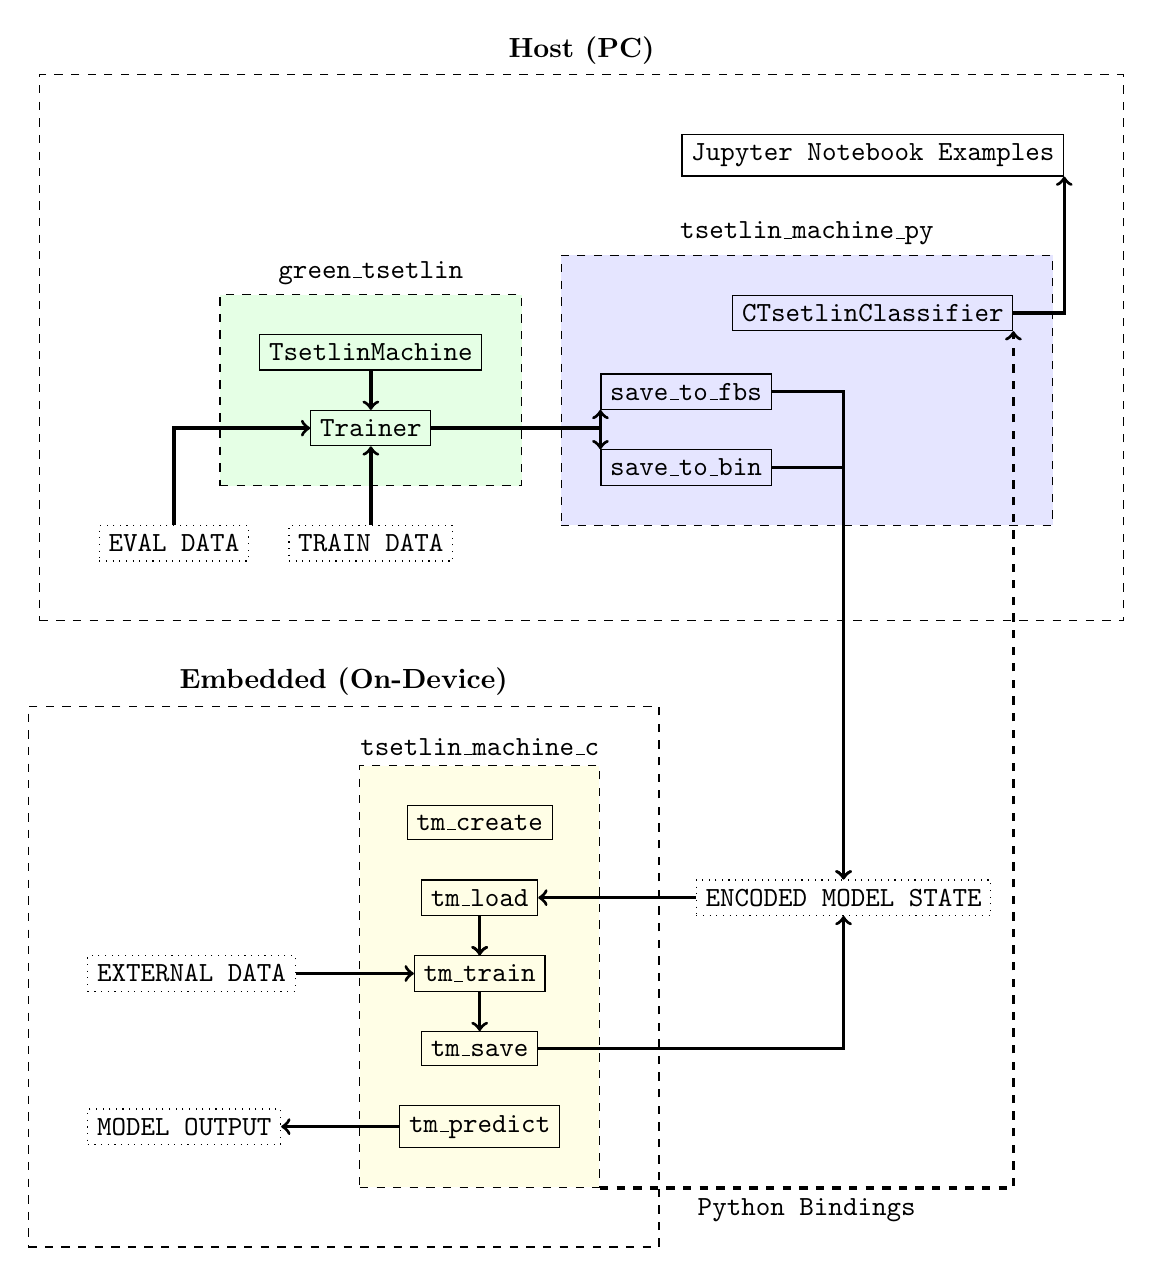
\begin{tikzpicture}
\pgfdeclarelayer{background}
\pgfsetlayers{background,main}

% --- host components (Main Layer) ---
\node [
    draw,
    rectangle,
] (tsetlinmachine) {\texttt{TsetlinMachine}};

\node [
    draw,
    rectangle,
    below=0.5cm of tsetlinmachine,
] (trainer) {\texttt{Trainer}};

\node [
    draw,
    dotted,
    rectangle,
    below=1cm of trainer,
] (traindata) {\texttt{TRAIN DATA}};

\node [
    draw,
    dotted,
    rectangle,
    left=0.5cm of traindata,
] (evaldata) {\texttt{EVAL DATA}};

\begin{pgfonlayer}{background}
\node [
    draw,
    dashed,
    rectangle,
    inner sep=0.5cm,
    fit=(tsetlinmachine) (trainer),
    label=above:\texttt{green\_tsetlin},
    fill=green!10,
] (greentsetlin) {};
\end{pgfonlayer}

\node [
    draw,
    rectangle,
    right=1.5cm of tsetlinmachine,
    yshift=-0.5cm,
] (savetofbs) {\texttt{save\_to\_fbs}};

\node [
    draw,
    rectangle,
    below=0.5cm of savetofbs,
] (savetobin) {\texttt{save\_to\_bin}};

\node [
    draw,
    rectangle,
    right=-0.5cm of savetofbs,
    yshift=1cm,
] (ctsetlinclassifier) {\texttt{CTsetlinClassifier}};

\node [
    draw,
    rectangle,
    above=1.5cm of ctsetlinclassifier,
] (jupyternotebook) {\texttt{Jupyter Notebook Examples}};

\node [
    draw,
    dotted,
    rectangle,
    below=5cm of savetobin,
    xshift=2cm,
] (modelstate) {\texttt{ENCODED MODEL STATE}};

\begin{pgfonlayer}{background}
\node [
    draw,
    dashed,
    rectangle,
    inner sep=0.5cm,
    label=above:\texttt{tsetlin\_machine\_py},
    fit=(savetofbs) (savetobin) (ctsetlinclassifier),
    fill=blue!10,
] (tsetlinmachinepy) {};
\end{pgfonlayer}

% --- host container ---
\node [
    draw,
    dashed,
    rectangle,
    fit=(greentsetlin) (tsetlinmachinepy) (traindata) (evaldata) (jupyternotebook),
    inner sep=0.75cm,
    label=above:\textbf{Host (PC)},
] (host) {};

% --- embedded component ---
\node [
    draw,
    rectangle,
    left=2cm of modelstate,
] (tmload) {\texttt{tm\_load}};

\node [
    draw,
    rectangle,
    above=0.5cm of tmload,
] (tmcreate) {\texttt{tm\_create}};

\node [
    draw,
    rectangle,
    below=0.5cm of tmload,
] (tmtrain) {\texttt{tm\_train}};

\node [
    draw,
    dotted,
    rectangle,
    left=1.5cm of tmtrain,
] (externaldata) {\texttt{EXTERNAL DATA}};

\node [
    draw,
    rectangle,
    below=0.5cm of tmtrain,
] (tmsave) {\texttt{tm\_save}};

\node [
    draw,
    rectangle,
    below=0.5cm of tmsave,
] (tmpredict) {\texttt{tm\_predict}};

\node [
    draw,
    dotted,
    rectangle,
    left=1.5cm of tmpredict,
] (modeloutput) {\texttt{MODEL OUTPUT}};

\begin{pgfonlayer}{background}
\node [
    draw,
    dashed,
    rectangle,
    inner sep=0.5cm,
    label=above:\texttt{tsetlin\_machine\_c},
    fit=(tmload) (tmtrain) (tmsave) (tmpredict) (tmcreate),
    fill=yellow!10,
] (tsetlinmachinec) {};
\end{pgfonlayer}

% --- embedded container ---
\node [
    draw,
    dashed,
    rectangle,
    fit=(tsetlinmachinec) (externaldata),
    inner sep=0.75cm,
    label=above:\textbf{Embedded (On-Device)},
] (embedded) {};

% --- connections ---
\begin{scope}[->, very thick]
\draw [->] (tsetlinmachine.south) -| (trainer.north);

\draw [->] (traindata.north) -| (trainer.south);
\draw [->] (evaldata.north) |- (trainer.west);

\draw [->] (trainer.east) -| (savetofbs.south west);
\draw [->] (trainer.east) -| (savetobin.north west);

\draw [->] (savetofbs.east) -| (modelstate.north);
\draw [->] (savetobin.east) -| (modelstate.north);

\draw [->] (ctsetlinclassifier.east) -| (jupyternotebook.south east);
\draw [->, dashed] (tsetlinmachinec.south east) -| (ctsetlinclassifier.south east) node[near start, below] {\texttt{Python Bindings}};

\draw [->] (modelstate.west) |- (tmload.east);
\draw [->] (tmsave.east) -| (modelstate.south);

\draw [->] (tmload.south) -| (tmtrain.north);
\draw [->] (tmload.south) -| (tmtrain.north);
\draw [->] (tmtrain.south) -| (tmsave.north);

\draw [->] (externaldata.east) |- (tmtrain.west);
\draw [->] (tmpredict.west) |- (modeloutput.east);
\end{scope}

\end{tikzpicture}

\caption[Project diagram]{Project diagram where \texttt{green\_tsetlin} is the external library with host and embedded parts separation.} % TODO: Add references to each block and briefly describe it; consider changing text to something more clear
\label{fig:projectdiagram}
\end{figure}


\newpage
\section{Competitive solutions}
According to the authors' knowledge, \GreenTsetlinName is the only production-ready implementation of the Tsetlin Machine. It is primarily a Python library with a C++ backend. A trained model can then be exported into a C header file and used for inference.  
This approach was found lacking in a number of ways;
\begin{enumerate}
    \item the exported model cannot be interpreted back to its previous form to perform modifications on it
    \item in particular, it makes training and fine-tuning the model impossible
    \item the model serialization is saved in a text format, which in this case allows inference without a separate interpreter, but otherwise means wasting a lot of storage space
\end{enumerate}

There are also numerous projects with far less mature implementations that were taken into consideration that didn't classify for this reason. [TODO: citations]

% Our solution aims to allow both inference and training, or on more resource constrained systems, just inference in (this is subject to debate) a more efficient format. 

% \section{Risk analysis}
% any?


% Przykład cytowania literatury~\cite{wilson2009prediction-interday}. Kolejny przykład
% cytowania kilku pozycji bibliograficznych~\cite{allen1999using-genetic, zitzler1999evolutionary-algorithms, pictet1995genetic-algorithms, wilhelmstotter2021jenetics, chmaj2015DistributedProcessingApplications}.

%%%%%%%%%%%%%%%%%%%%%%%%%%%%%%%%%%%%%%%%%%%%%%%%%%%%%%%%%%%%%%%%%%%%%%%%%%%%%%%
\chapter{\ChapterTitleTheory}
\label{sec:theoretical-background}
This chapter introduces the Tsetlin Machine, a method for pattern recognition based on propositional logic and game theory. We briefly examine the ideas developed in the original research~\cite{granmo2021tsetlinmachinegame, glimsdal2021coalescedmultioutputtsetlinmachines} that were necessary for our work, explaining how the model is designed from the ground up. Finally, we discuss scenarios where this approach has the potential to be a viable alternative to neural networks. For a more extensive introduction to Tsetlin Machines, refer to~\cite{granmo2022tsetlinmachinebookchap1, granmo2022tsetlinmachinebookchap2}.

\section{Tsetlin Machine Overview}
The emergence of the Tsetlin Machine is rooted in the development of a lesser-known, yet fundamental and versatile learning mechanism called the Tsetlin Automaton, developed by M.L. Tsetlin in the early 1960s~\cite{granmo2021tsetlinmachinegame, tsetlin1961behaviour}. Further research on this topic proposes a novel technique for complex large scale classification constructed using Tsetlin Automata~\cite{granmo2021tsetlinmachinegame}.

\paragraph{Pattern Recognition}
The most important distinction of the Tsetlin Machine lies in how it addresses pattern recognition problems. While the precision of a machine learning technique is related to its capability to represent patterns, the Tsetlin Machine decomposes complex problems into self-contained sub-patterns~\cite{granmo2021tsetlinmachinegame}. Instead of using the complex arithmetic found in neural networks, this method utilizes Boolean algebra, which is the basis of how digital computers operate. As a result, the machine captures the structure of the data by expressing patterns as conjunctive clauses in propositional logic.

\paragraph{Logic-Based Approach}
The Tsetlin Machine processes input features as bits to construct propositional logic expressed as "If-Then" rules, which offers both computational simplicity and interpretability.
In short, given an input vector of propositional variables $X = (x_1, \dots, x_n) \in \{0,1\}^n$, we add their negated counterparts $\overline{x}_k = 1 - x_k$ to build a set of literals $L = \{l_1 \dots, l_{2n}\}$. From these literals, we construct conjunctive clauses that determine the output vector $Y = (y_1, \dots, y_m) \in \{0,1\}^m$. For example, clause $C(X) = x_1 \land x_2 = x_1 x_2$ consists of literals $\{x_1, x_2\}$ and outputs $1$ if and only if $x_1 = x_2 = 1$~\cite{granmo2021tsetlinmachinegame}. The simple inference structure of the Tsetlin machine can be seen in Figure \ref{fig:tsetlinmachinestructure}.

\begin{figure}[!htbp]
    \centering
    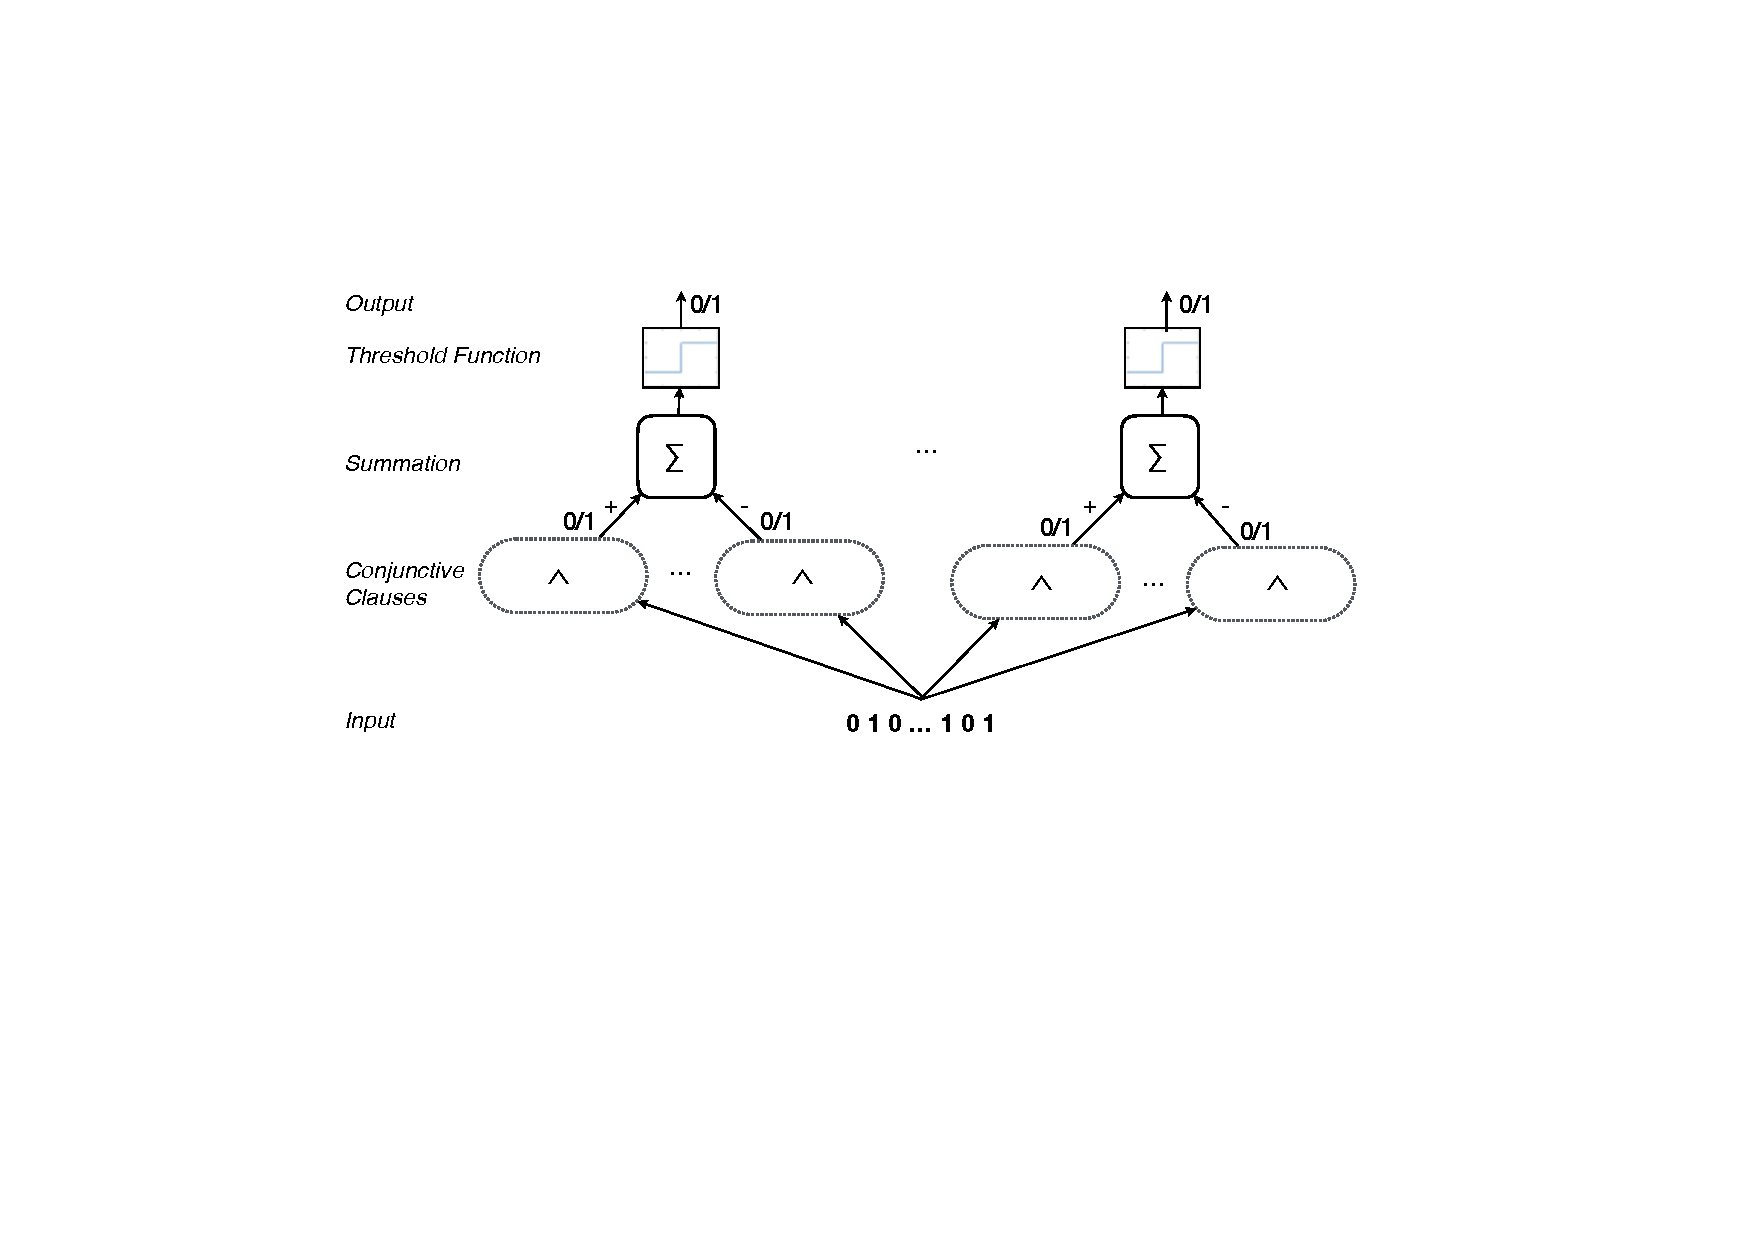
\includegraphics[width=.9\textwidth]{images/Overall_Architecture_Summation[1804.01508v15].pdf}
    \caption[The Tsetlin Machine inference structure]{The Tsetlin Machine inference structure (source: \cite{granmo2021tsetlinmachinegame})}
    \label{fig:tsetlinmachinestructure}
\end{figure}

\section{Tsetlin Automaton}

\paragraph{State-Based Memory}
% - Solves simple choice problem
% - Construction based on Finite State Machine
% - Uses single integer index to track memory
\paragraph{Decision Making}
% - The automaton based on its state (memory) decides between "Include" and "Exclude" action

\begin{figure}[!htbp]
    \centering
    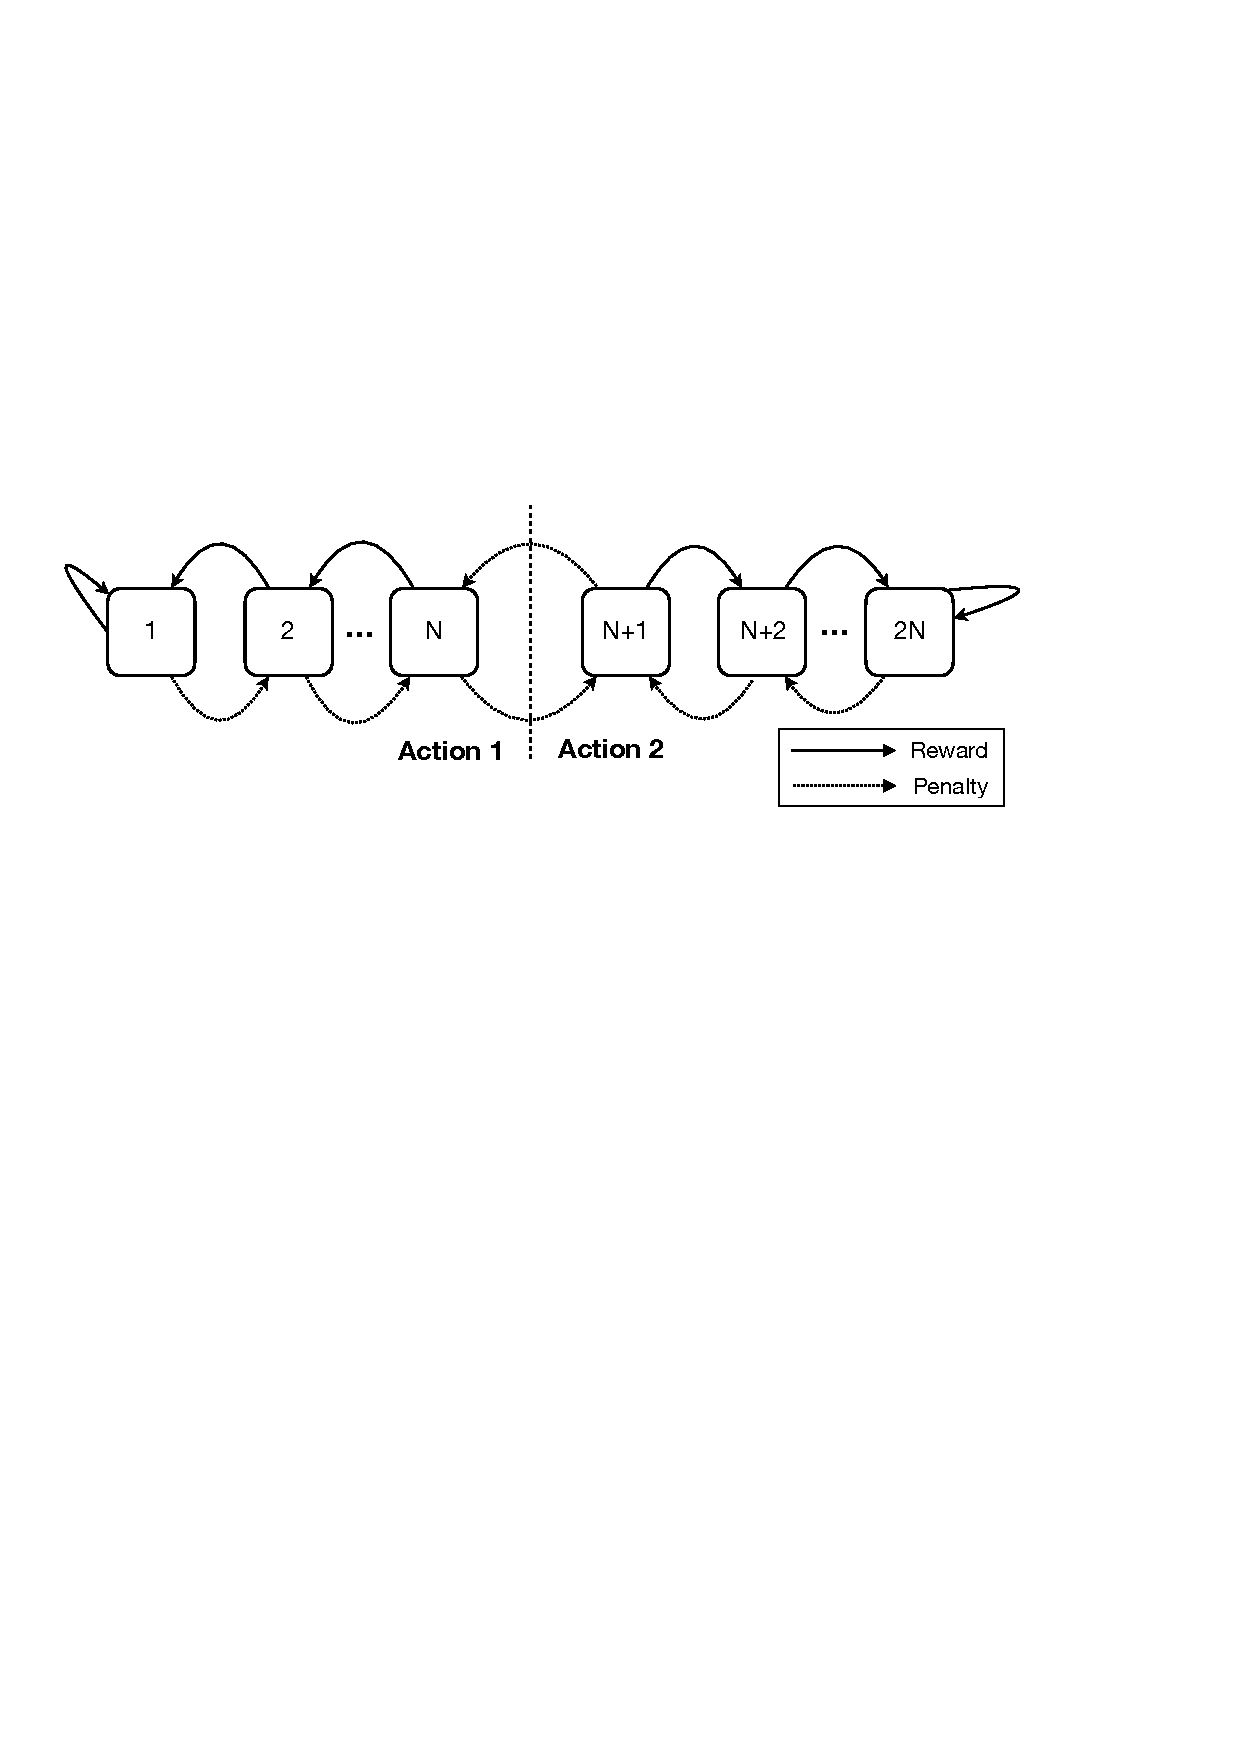
\includegraphics[width=.9\textwidth]{images/Tsetlin_Automaton_Generic[1804.01508v15].pdf}
    \caption[A Tsetlin Automaton for two-action environment]{A Tsetlin Automaton for two-action environment (source: \cite{granmo2021tsetlinmachinegame})}
    \label{fig:tsetlinautomatongeneric}
\end{figure}

\section{Architecture and Problem Representation}

\paragraph{Rule Construction}
% - Teams of automata are grouped into "Clauses" (AND rules) (example: wheels and not wings and doors)
% - Complex data can be broken into simpler patterns
\paragraph{Class Prediction by Voting}
% - Positive clauses vote for specific class and negative clauses vote against
% - Needs to distinguish noise and data
\paragraph{Binarization of Data}
% - This approach requires turinging real-world data into binary format that is the input to the machine

\begin{figure}[!htbp]
    \centering
    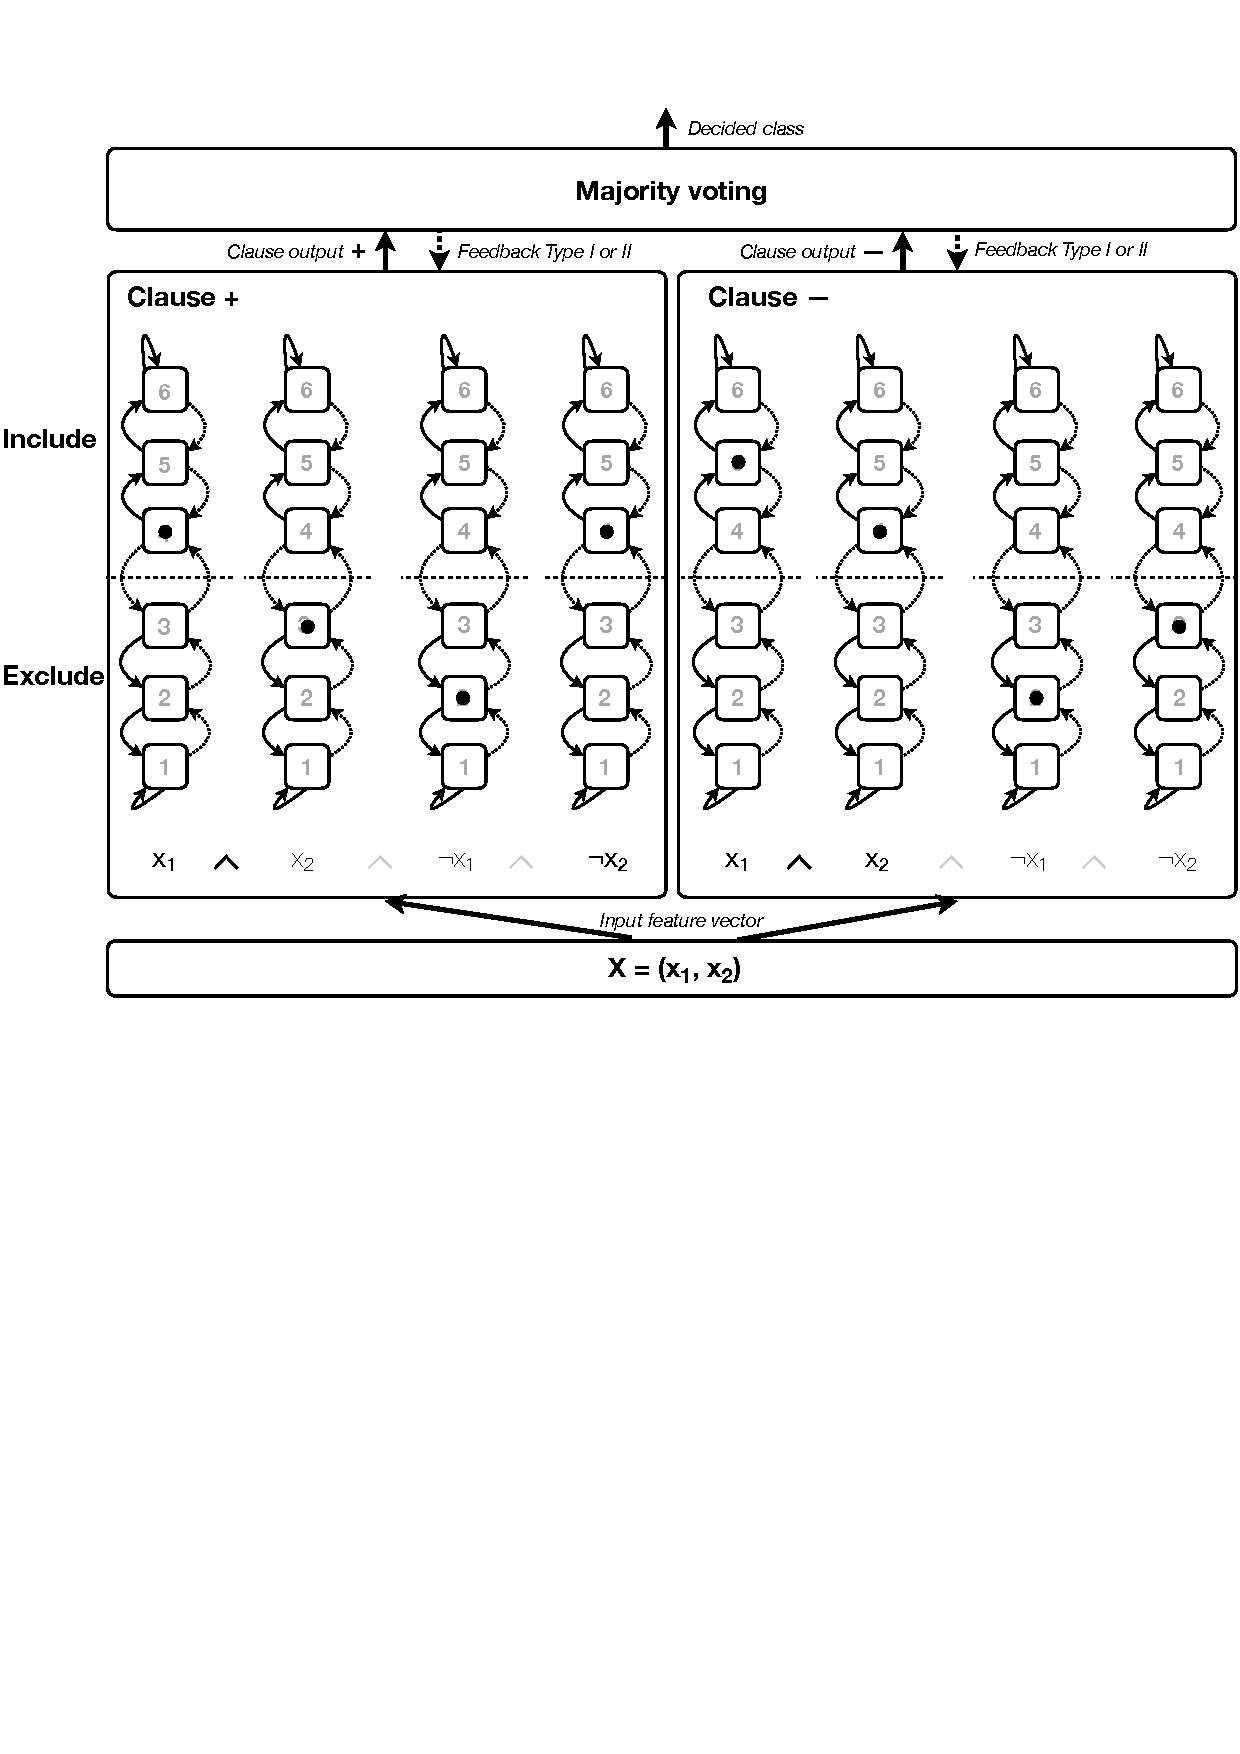
\includegraphics[width=.9\textwidth]{images/Tsetlin_Machine_Example_Configuration_Full[1804.01508v15].pdf}
    \caption[Two Tsetlin Automata teams]{Two Tsetlin Automata teams, each producing a conjunctive clause (source: \cite{granmo2021tsetlinmachinegame})}
    \label{fig:tsetlinmachineconfiguration}
\end{figure}

\begin{figure}[!htbp]
    \centering
    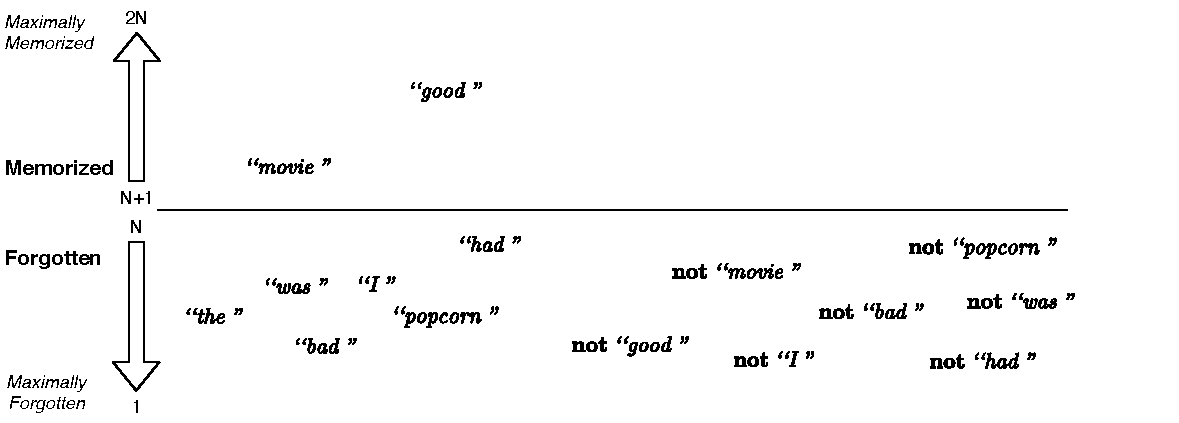
\includegraphics[width=.9\textwidth]{images/Memory_IMDb[2108.07594v1].pdf}
    \caption[Sticky memory for IMDb example]{Sticky memory for IMDb example with depth N for the clause: "good" AND "movie" (source: \cite{glimsdal2021coalescedmultioutputtsetlinmachines})}
    \label{fig:memoryimdb}
\end{figure}

\section{Learning Algorithm}
\paragraph{Addressing False Negatives (Type I Feedback)}
% - Recognize Feedback
\paragraph{Addressing False Positives (Type II Feedback)}
% - Erase Feedback

\begin{figure}[!htbp]
    \begin{center}
        \subfigure[Type Ia feedback triggered by input "The movie was good, and I had popcorn."]{%
        \label{fig:memoryimdbtypeIa}
        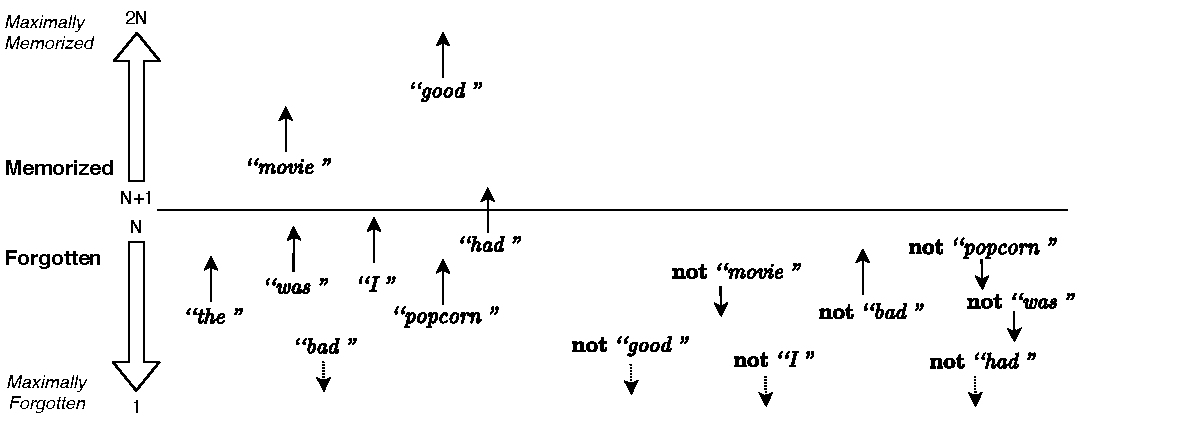
\includegraphics[width=.9\textwidth]{images/Memory_IMDb_Type_Ia[2108.07594v1].pdf}}%
        \\
        \subfigure[Type Ib feedback triggered by input "Was good, and I had popcorn."]{%
        \label{fig:memoryimdbtypeIb}
        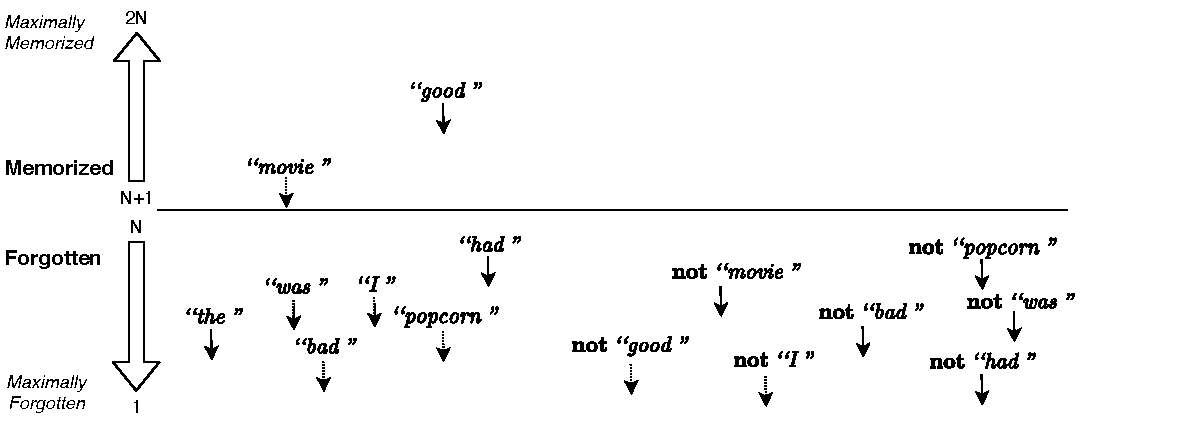
\includegraphics[width=.9\textwidth]{images/Memory_IMDb_Type_Ib[2108.07594v1].pdf}}%
        \\
        \subfigure[Type II feedback applied to input "The movie was bad, and I had popcorn."]{%
        \label{fig:memoryimdbtypeII}
        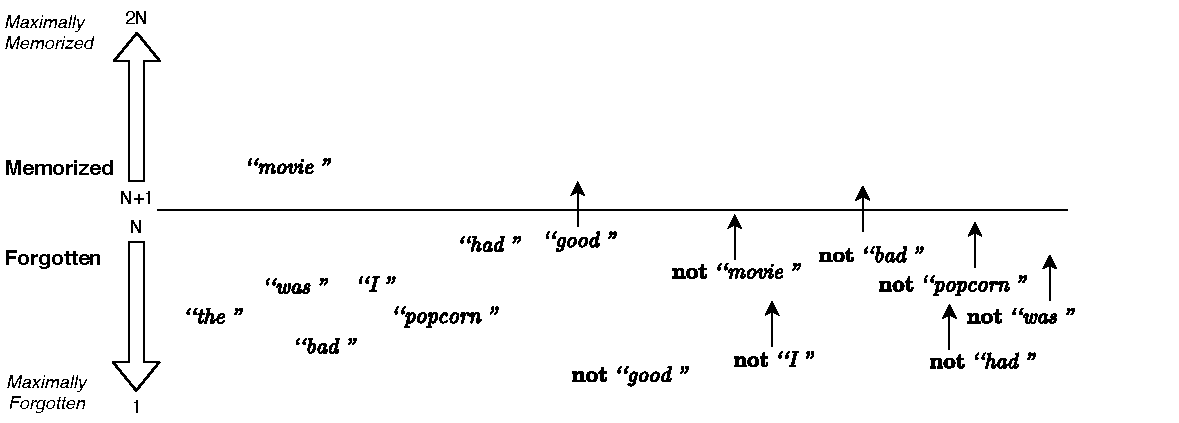
\includegraphics[width=.9\textwidth]{images/Memory_IMDb_Type_II[2108.07594v1].pdf}}%
    \end{center}
    \caption[Comparison of feedback types for IMDb example]{Comparison of feedback types Ia, Ib, and II for IMDb example (source: \cite{glimsdal2021coalescedmultioutputtsetlinmachines})}
    \label{fig:memoryimdbtypes}
\end{figure}

\section{Tsetlin Machine Variants}
\paragraph{Standard Dense Architecture}
\paragraph{Sparse Architecture}
% - removes automata that are not contributing
\paragraph{Stateless Inference Model}
% - saves memory when required only on predictions

\section{Comparison with Neural Networks}

% moje 2 grosze
% https://arxiv.org/abs/2212.13634
% TM używa w większości algebry całkowitoliczbowej nie floatów co może być bardzo atutem na niektórych platformach, szczególnie takich co procesor nie ma operacji na floatach w ogóle
% problem 1 - no tyle że nie lol bo jednak używa floatów (czego dało by się pozbyć, patrz further work w ostatnim rozdziale)
% problem 2 - z punktu hardwareowej optymalizacji, mimo że floaty są bardzo kosztowne, to ich algebra i bardzo dziwne sposoby optymalizacji są giga zoptymalizowane (temu że tyle kosztowały a całe ML na nich stoi) i to tak mocno że teraz to algebra na intach się nie opłaca

\paragraph{Transparent Logic}
% - Learned logic is human readable (If X and not Y then Z) compared to Black Box approach of neural networks
\paragraph{Energy Efficiency}
% - More optimizations possible when working with logic operations like AND/OR/NOT, compared to float operations on Neural Networks
\paragraph{Performance with Training Data}
% - (cite) TM often require less training data to reach high accuracy

\begin{figure}[!htbp]
    \centering
    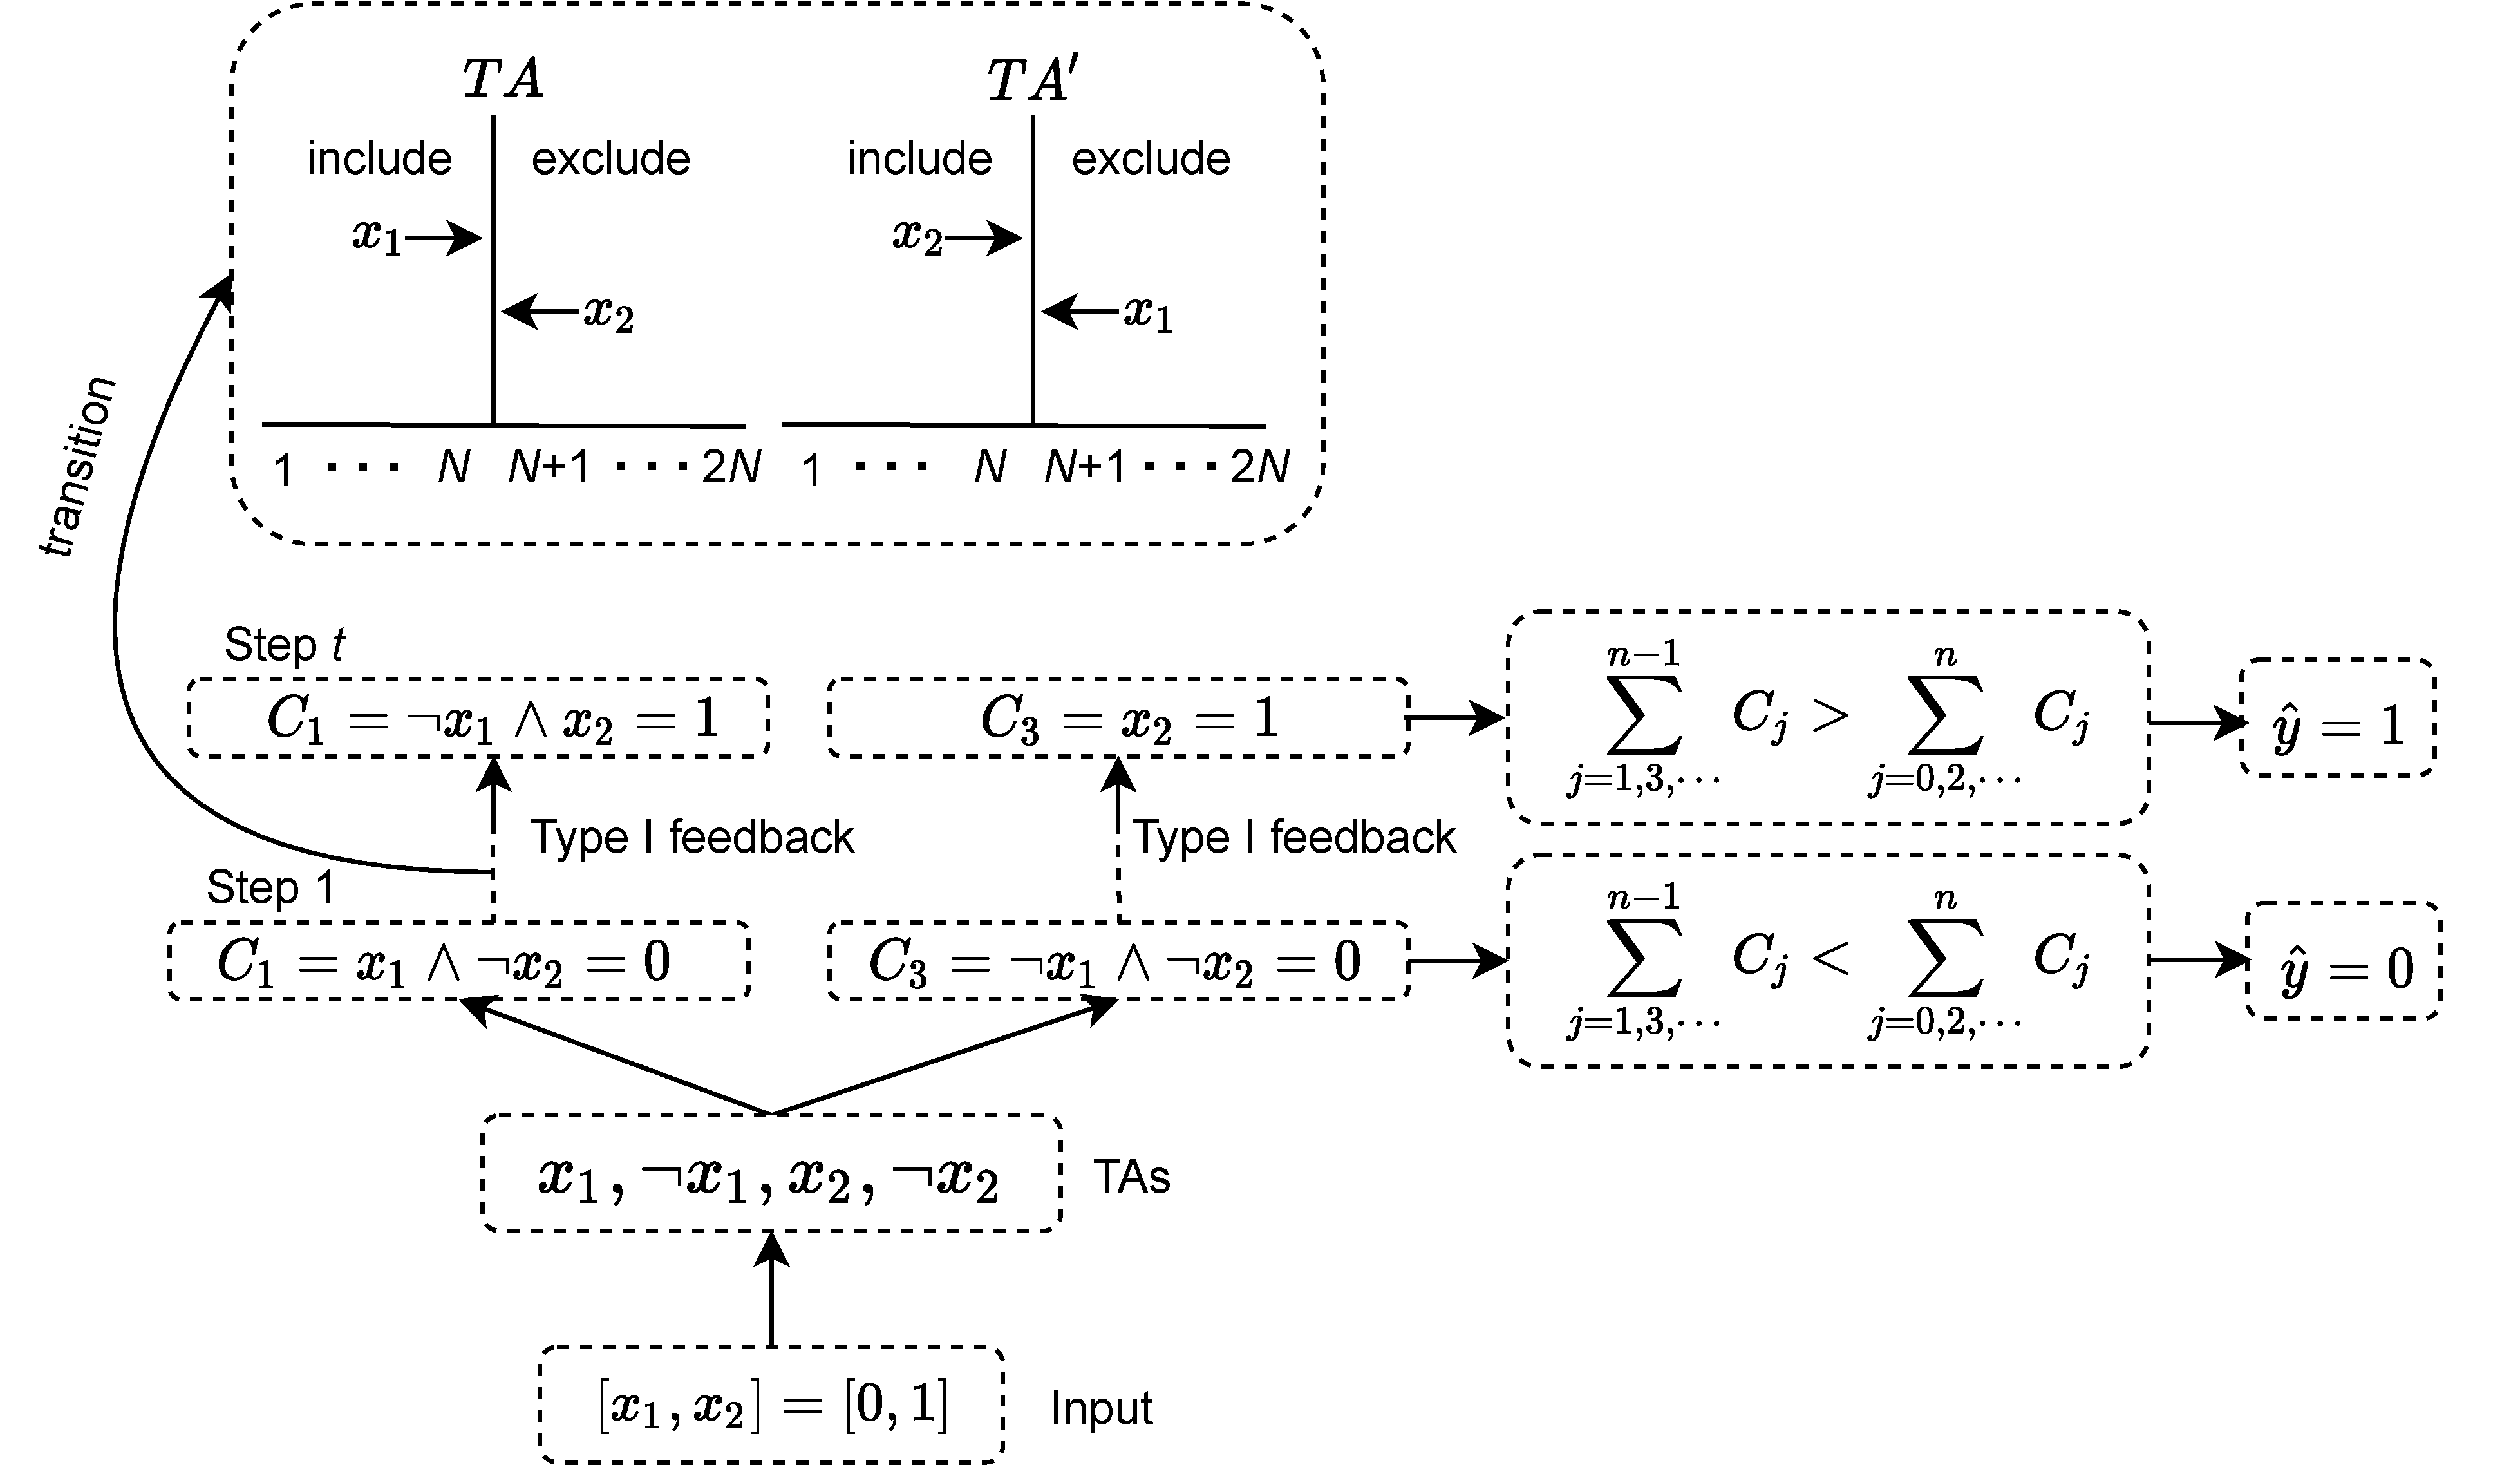
\includegraphics[width=.9\textwidth]{images/TM[arXiv-2212.13634v1].pdf}
    \caption[Tsetlin Machine XOR-gate training]{Tsetlin Machine learning dynamics for an XOR-gate training sample, with input $(x_1 = 0, x_2 = 1)$ and output target $y = 1$ (source: \cite{sharma2022equivalenceweightedtsetlinmachine})}
    \label{fig:tsetlinmachinexorgate}
\end{figure}

%%%%%%%%%%%%%%%%%%%%%%%%%%%%%%%%%%%%%%%%%%%%%%%%%%%%%%%%%%%%%%%%%%%%%%%%%%%%%%%
\chapter{\ChapterTitleScope}
\label{sec:functional-scope}

% poniższą zawartość rodziału należy usunąć z finalnej wersji pracy.
% \emph{Kontekst użytkowania produktu (aktorzy, współpracujące systemy) oraz specyfikacja wymagań funkcjonalnych i niefunkcjonalnych.}

This chapter outlines the considerations and requirements for the library. Describes the intended audience and details the key decisions made during development. These choices are further described in subsequent sections on Functional and Non-functional requirements.

\section{Target audience}
Due to the experimental nature of this work, the key design goal was to make the library both easy to use and easy to understand. This is necessary as we anticipate that users may need to adapt the library for integration into their specific applications.

\paragraph{Embedded Developers}
The library was designed with the limitations of embedded hardware in mind. Unlike many alternatives, it supports every step of the process on-device, while others implement predictions on-device only. Thanks to the designed model exchange format, users can choose to train models on faster hardware or use the \GreenTsetlinName library to later move them to the edge device. Additionally, the efficiency gains promised by Tsetlin Machines~\cite{granmo2021tsetlinmachinegame} are highly beneficial for these resource limited devices, where standard machine learning methods are often too expensive or complicated to run.

\paragraph{Researchers}
As Tsetlin Machines have only recently started getting more recognition we expect the researchers familiar with classic machine learning models to benefit from being able to implement them in their workflows. Making the library's interface familiar to them allows for rapid prototyping which differs our solution from others which require more domain knowledge. This in turn makes it easier to benchmark them in various potential use cases.


\section{Functional requirements}

\paragraph{On-device Training and Inference}
Our solution was designed to support all steps of a Tsetlin Machine model directly on target hardware. Unlike other embedded machine learning frameworks that perform only inference on edge devices, this library enables the model to learn directly from newly gathered data. This is necessary for applications that adapt to local sensor data without a constant connection to the central server.

\paragraph{Interoperability and Serialization}
The library must implement functionality for saving and loading model states. This requires a standardized serialization format to ensure compatibility with the \GreenTsetlinName library. This compatibility is essential for the users to leverage high-performance workstations to pre-train models, export them, and then deploy them directly to the embedded devices. Furthermore, models trained or tuned on the edge must also be exportable for backup or analysis on faster hardware.

\paragraph{Configurable Hyperparameters}
Exposing Tsetlin Machine model hyperparameters is necessary for fitting the model to its application with varied limitations dictated by hardware or the input data itself. Researchers and developers must be able to easily fine-tune these parameters when designing their solution for each specific problem. This allows optimization of performance, memory footprint, or accuracy without modifying library code. 

\paragraph{Correctness with the Theoretical Work}
The implementation must behave as described in theoretical research~\cite{granmo2021tsetlinmachinegame}. It is required to accurately model the Tsetlin Automata logic and implement the specific learning rules (Type I and Type II feedback) defined in the original papers. This ensures that the software is a close representation of the method proposed in the theory and avoids unintended assumptions.


\section{Non-functional requirements}

\paragraph{Portability}
The library must be designed for compatibility, avoiding dependencies on any specific hardware or operating system. The functionality of the external library should be defined during compilation if there is a risk that it may not work on the desired target. This strategy ensures that the code can be compiled with minimal, if any, modifications for a wide range of hardware architectures. The resulting portability, coupled with the adjustable model parameters, allows end users to create a solution that is both widely adoptable and future-proof.

\paragraph{Performance and Memory Usage}
Optimizations are significantly beneficial, as the library's performance impacts both the training step and, more importantly, the real-time predictions on target devices. Given that Tsetlin Machines heavily rely on binary logic and random number generators, optimizing these areas allows for better utilization of limited hardware resources. This optimization extends to memory management, since the memory is needed to store the model on the device, as well as the memory used during runtime, must also be considered.

\paragraph{Simple API}
The Applications Programming Interface (API) must be intuitive and well-documented. Its design should follow standard interfaces developed by major machine learning libraries, allowing users unfamiliar with Tsetlin Machine theory to quickly prototype concepts. This simple interface allows a developer to easily integrate the library into an existing project. Moreover, supporting quick prototyping in environments like Python Jupyter Notebooks alongside established models from libraries such as Scikit-learn speeds up development before deployment to embedded devices.

\paragraph{Testing and Examples}
As with any software project, testing enhances the development process and maintenance. Code examples provide a starting point for users unfamiliar with the project. Furthermore, simple installation and easy to run examples encourage potential users to quickly try the library. Finally, these tests help verify that the library runs correctly on new devices with different hardware limitations.


%%%%%%%%%%%%%%%%%%%%%%%%%%%%%%%%%%%%%%%%%%%%%%%%%%%%%%%%%%%%%%%%%%%%%%%%%%%%%%%
\chapter{\ChapterTitleRealizationAspects}
\label{sec:realization-aspects}

% poniższą zawartość rodziału należy usunąć z finalnej wersji pracy.
\emph{Przyjęte założenia, struktura i zasada działania systemu, wykorzystane rozwiązania technologiczne wraz z uzasadnieniem ich wyboru, istotne mechanizmy i zastosowane algorytmy.}

This section describes the design choices of \LibraryName as well as the rationale behind them, and the overarching architecture of the solution. The actual Tsetlin Machine implementation is described in detail to make it intuitive. It describes used tools, solutions and algorithms. Additionally, it discusses several interesting problems that were encountered.

\section{Design}
Even though optimization was the primary objective, not every method could be utilized due to the target environments having very limited resources and hardware limitations. In particular, vectorization was completely out of the picture, even though \GreenTsetlinName has it enabled by default. GPU programming was obviously dismissed for the same reason - although notably, such an implementation is possible. % TODO: citation for cuda project

\subsection{Programming language}
Since the thesis topic requires \LibraryName to be designed for embedded devices, there were only a few suitable options like C/C++, Rust or MicroPython. C was chosen as the most widely used language for embedded systems - it is efficient, lightweight and portable. It's popularity also means it has extensive third party library support. The authors' previous experience working with C/C++ also influenced this decision.  
Exporting models from \GreenTsetlinName is done in Python, as it is a Python library.  
\LibraryName also has Python bindings so that it can be used conveniently from Python.

\subsection{Execution engine}
Even though there exists a number of existing libraries implementing the Tsetlin Machine, \LibraryName was essentially created from the ground up without taking much inspiration or hints from them. It was required to be written primarily with optimization in mind so that it works as fast as possible while maintaining small size and portability on top of utilizing little power and memory. \\
It was also decided \LibraryName should support multiple different Tsetlin Machine variants so their efficiency could be tested - Coalesced, Sparse and Stateless.

\newpage
\subsection{Model serialization library}
Several libraries were compiled and compared as possible options to implement the model serialization format. Only C libraries were taken into consideration. See table ~\ref{tab:serial-lib-comp}
% TODO: czemu to nie jest 4.1
\begin{table}[h]
\centering
\begin{tabularx}{\textwidth}{
  | >{\raggedright\arraybackslash}X 
  | >{\raggedright\arraybackslash}X 
  | >{\raggedright\arraybackslash}X 
  | >{\raggedright\arraybackslash}X 
  | >{\raggedright\arraybackslash}X |
}
\hline
Format name & Comment & Schema complexity & Efficiency on edge device & Library size on edge device \\
\hline
Protocol Buffers & Simple and small model representation & Low & Fast but needs object parsing & Too big \\
\hline
ONNX & A standardized way to store models and operation graphs & High & Low - needs graph and tensor parsing & Much too big \\
\hline
FlatBuffers & "Protocol buffers lite" & Low & Very fast, zero-copy & Acceptable \\
\hline
\end{tabularx}
\caption{Comparison of selected model serialization libraries}
\label{tab:serial-lib-comp}
\end{table}


\subsection{Concept of the solution}
move here, describe


\subsection{Tsetlin Automaton}
A Tsetlin Automaton is the smallest part of a Tsetlin Machine, and it is what clauses consist of. Implementation-wise it is represented by a singular, 8-bit integer, meaning its values can range from -127 to 127 by default. The range can be made smaller by setting model parameters $max\_state$ and $min\_state$ \\
Further on in this thesis, the term that a Tsetlin Automaton is active, means its internal integer value is greater or equal than halfway between $max\_state$ and $min\_state$; $value \ge \frac{max\_state + min\_state}{2}$  \\
One input bit on position $i$ has two corresponding Tsetlin Automata at positions in clause $2 \times i$ and $2 \times i + 1$. The first one -- positive -- decides whether the input bit -- $x_i$ -- should be included in the clause, and the other -- negative -- whether its negation -- $\neg x_i$ -- should be included.


\section{Coalesced Tsetlin Machine}
Coalesced Tsetlin Machine is the variant most closely resembling the original Tsetlin Machine out of those implemented by \LibraryName. The implementation closely follows the paper.~\cite{glimsdal2021coalescedmultioutputtsetlinmachines}


\subsection{Training}
The training loop consists of three distinct steps repeated for each datapoint.
\begin{enumerate}
    \item Calculate clause output
    \item Sum votes
    \item Calculate and apply feedback
\end{enumerate}

\subsubsection{Calculate clause output}
The current states of Tsetlin Automata in each clause are used to determine whether the clause activates - 1, or not - 0. This output is temporarily stored in an internal array. \\
For this step specifically, a clause is active if either of two conditions is met:
\begin{itemize}
    \item \textbf{the clause is empty} - no Tsetlin Automaton is active
    \item for the training input datapoint, all bits corresponding to active positive Tsetlin Automata of this clause are set and all bits corresponding to active negative Tsetlin Automata of this clause are unset
\end{itemize}

\subsubsection{Sum votes}
This step uses the information calculated in the previous point whether clauses are active or not. Active clauses vote for all possible classes with trained weights. Specifically, clause $i$ votes for class $j$ with trained weight $w_{i,j}$. $w_{i,j}$ can be positive or negative.\\
As all active clauses vote, each class accumulates their votes. The sum of votes is then clipped to parameter $treshold$. It serves the same purpose as gradient clipping in other ML architectures, mainly for numerical stability. %TODO: citation

\subsubsection{Calculate and apply feedback}
As the sum of votes indicates whether a class should be chosen or not, that prediction can be compared to the actual datapoint label. Based on this information, a suitable feedback to be applied to Tsetlin Automata. \\
For each datapoint two classes are specified for feedback
\begin{enumerate}
    \item positive - one of the classes, or the one class, specified by label
    \item negative - one of the classes not specified by label
\end{enumerate}
Both have a chance to trigger feedback to all clauses. \\
For the positive class, the chance is inversely proportional to the clipped sum of votes it received. That means the model applies feedback more often the \textit{less} sure it is the class is correct. Although unintuitive at first, this practice is used to avoid overfitting. \\
For the negative class, the chance is proportional to the clipped sum of votes it received. This means the model applies feedback more often the more sure it is the class is incorrect. \\

\paragraph{Customization}
What is unique to \LibraryName, it allows both predictions and output to be customized to be virtually anything. \\
A custom feedback function can be set for the model, to override how positive and negative classes are chosen. The default uses normal classification, where the output and prediction is an integer identifying a class. \\
Another predefined function allows multi-class classification, where output and prediction is an 8-bit integer array where the length is the number of classes, where value 1 signifies a class with a given identifier being chosen, value 0 - not chosen. \\
\vspace{7pt}
Also a custom comparison function can be set for the model, to override when the output and prediction data classes should be treated as equal. By default a simple memory comparison is used, which handles the vast majority of uses -- even when fully customized.

\subsubsection{Feedback}
\label{feedback-dense}
When a chosen class triggers feedback to all clauses, for each clause separately one of three feedback types may be applied. \\
Tsetlin Automata changes specified in \textbf{Action} aren't always changed -- they have a random chance to do so based on the parameter \textit{s} -- sensitivity -- further explained in \textbf{Sensitivity} for each feedback type. \\

\paragraph{Type Ia}
\begin{description}
    \item[Condition] the clause is active and voted correctly for the chosen class (with the correct weight sign)
    \item[Action] reinforce Tsetlin Automata making up the clause, reinforce weight for the chosen class
    \item[Sensitivity] the chance for change is either \( \frac{1}{s} \) for true positive and true negative Tsetlin Automata, and otherwise its inversion -- \( \frac{s - 1}{s} \). Model parameter \textit{boost\_true\_positive} makes it so that true positive Tsetlin Automata are always changed.
    \item[Intuition] the clause should continue to vote for the same class
\end{description}

\paragraph{Type Ib}
\begin{description}
    \item[Condition] the clause is inactive and (would have) voted correctly for the chosen class
    \item[Action] lower the confidence of all the Tsetlin Automata making up the clause, positive and negative
    \item[Sensitivity] the chance for change is always \( \frac{1}{s} \)
    \item[Intuition] the clause should "find something else to do", countering force
\end{description}

\paragraph{Type II}
\begin{description}
    \item[Condition] the clause is active and voted incorrectly for the chosen class
    \item[Action] raise, towards activation, inactive Tsetlin Automatons that could deactivate the clause for this datapoint, punish the weight of the chosen class towards zero
    \item[Sensitivity] change always happens
    \item[Intuition] try two things at once: exclude the clause and fix the weight (flip the sign). Although these goals are opposing, just one of them needs to come true, and the hope is one of them should do so before the other.
\end{description}

Nothing happens if the clause if inactive and would have voted incorrectly.

\subsection{Inference}
Inference on a datapoint looks very similar to training, with few key differences.
\begin{enumerate}
    \item Calculate clause output
    \item Sum votes
    \item Apply output activation
\end{enumerate}

\subsubsection{Calculate clause output}
Unlike in training, an empty clause -- with no active Tsetlin Automata -- is inactive. Otherwise it does the same thing -- calculates which clauses are active with a given input.

\subsubsection{Sum votes}
Exactly the same as training. Sums up class votes from active clauses.

\subsubsection{Apply output activation}
Applies a function to determine the output from the summed up class votes. By default, it simply returns an integer -- an identifier of a class with the most votes.

\paragraph{Customization}
Again, this can be fully customized. A custom output activation function can be set for the model, to override what the model outputs based on the summed up weights. \\
Another predefined function allows multi-class classification, where the output is an 8-bit integer array where the length is the number of classes, where value 1 signifies a class with a given identifier being chosen, value 0 - not chosen.

\subsection{Model serialization format}
TODO

\section{Sparse Tsetlin Machine}
A Sparse Tsetlin Machine~\cite{glimsdal2024sparsetsetlinmachine} 

\subsection{Model serialization format}

\section{Stateless}
\subsection{Model serialization format}

\section{Optimizations}
Seeing as speed, size, portability as well as limiting the usage of power and memory were all key requirements, optimizations were the main focus of this thesis. In this section a few of the more interesting examples are listed.

\subsection{Pseudo random number generation}
Analyzing the efficiency of a development version with valgrind and callgrind, it was obvious that most training time was spent on calls to \textit{rand()} - pseudo random number generation. \\
While it isn't costly to call once, the cost quickly accumulates over millions of calls.

\subsubsection{Analysis}
\textit{rand()} is costly because it aims for a uniform spread, as evenly as possible. \LibraryName doesn't care that much as the deviation spreads across millions of calls - but it does very much care for speed and lower power usage. The pseudo random number generation for this purpose doesn't need to by cryptographically secure either -- \textit{rand()} isn't anyways. \\
A quick look at \GreenTsetlinName revealed that it suffered from the same problem. Its solution was to use a wyhash64 algorithm. Using just an 64-bit integer addition, two 128-bit integer multiplications and few bitwise operations as well as a double multiplication, it is overall a much cheaper solution.\\
Listing ~\ref{lst:wyhash64} shows the \GreenTsetlinName implementation of wyhash64.
\begin{lstlisting}[language=C,caption={[\GreenTsetlinName implementation of wyhash64]\GreenTsetlinName implementation of wyhash64},label=lst:wyhash64]
double next_u()
{
    wyhash64_x += 0x60bee2bee120fc15;
    __uint128_t tmp;
    tmp = (__uint128_t) wyhash64_x * 0xa3b195354a39b70d;
    uint64_t m1 = (tmp >> 64) ^ tmp;
    tmp = (__uint128_t)m1 * 0x1b03738712fad5c9;
    uint64_t m2 = ((tmp >> 64) ^ tmp);

    double r = 0x1.0p-64 * m2;
    return r;
}
\end{lstlisting}

\subsubsection{Solution}
Wyhash64 is a much cheaper solution, but it's still not cheap. 128-bit integer multiplications and double multiplication cost many precious CPU cycles which means time and power. \\
Listing ~\ref{lst:fast-prng} shows the \LibraryName implementation of xorshift32. \\
All that's really needed is a few bit shifts and XOR operations. It uses so few CPU cycles it's basically free. It might also be the case one of the authors likes low-level optimization an unhealthy amount. 

\begin{lstlisting}[language=C,caption={[\LibraryName implementation of xorshift32]\LibraryName implementation of xorshift32},label=lst:fast-prng]
uint32_t prng_next_uint32(struct FastPRNG* prng) {
    uint32_t x = prng->state;
    x ^= x << 13;
    x ^= x >> 17;
    x ^= x << 5;
    prng->state = x;
    return x;
}

float prng_next_float(struct FastPRNG* prng) {
    uint32_t x = prng->state;
    x ^= x << 13;
    x ^= x >> 17;
    x ^= x << 5;
    prng->state = x;

    static union {
        uint32_t u32;
        float f;
    } caster;

    /* Reinterpret x as float: keep random mantissa, set exponent to 127
       (1.0f), then subtract 1.0f to obtain value in [0,1). */
    caster.u32 = 0x3F800000 | x >> 9;

    return caster.f - 1.0f;
}
\end{lstlisting}


%%%%%%%%%%%%%%%%%%%%%%%%%%%%%%%%%%%%%%%%%%%%%%%%%%%%%%%%%%%%%%%%%%%%%%%%%%%%%%%
\chapter{\ChapterTitleWorkOrganization}
\label{sec:work-organization}

% poniższą zawartość rodziału należy usunąć z finalnej wersji pracy.
\emph{Struktura zespołu (role poszczególnych osób), krótki opis i uzasadnienie przyjętej metodyki i/lub kolejności prac, planowane i zrealizowane etapy prac ze wskazaniem udziału poszczególnych członków zespołu, wykorzystane praktyki i narzędzia w zarządzaniu projektem.}

Mention development and research (to even start development for one)

\section{Team members and their roles}

\paragraph{Igor Sikora} - C implementation of the Tsetlin Machine execution engine, correctness tests, optimizations

\paragraph{Robert Mesek} - Python bindings and examples, benchmarks, CI/CD, integration with FlatBuffers

\section{Work planning and order of tasks}
the whole saga on dc

\section{Used tools}

\paragraph{Git} gud

\paragraph{GitHub} - popular hosting service for git

\paragraph{valgrind with callgrind} my beloved

\paragraph{Visual Studio Code} - versatile, lightweight, free

\paragraph{Cmake} - like make but worse :p

\paragraph{Discord} - group communication; texting, voice and video calls, free, conversations separated between thematic channels and threads

\paragraph{MS Teams} - communication with project supervisor

\paragraph{Email} - communication with project supervisor

\paragraph{Overleaf} - free online \LaTeX editor

\paragraph{arXiv} - searching for and viewing scientific papers on the Tsetlin Machines


% \section{Used methodologies}
  
%%%%%%%%%%%%%%%%%%%%%%%%%%%%%%%%%%%%%%%%%%%%%%%%%%%%%%%%%%%%%%%%%%%%%%%%%%%%%%%
\chapter{\ChapterTitleDocumentation}
\label{sec:documentation-usage}

The \LibraryName library is a low-level C implementation of the Tsetlin Machine. It is optimized for speed and size, making it suitable for environments with limited resources. It comes with a model serialization format designed to minimize model size and a way to convert existing \GreenTsetlinName models to this format. It is also possible to use \LibraryName conveniently from Python with the same syntax as many popular Machine Learning libraries thanks to its python bindings.

\section{Quick start - C}

Listing ~\ref{lst:example-c} shows the basic usage of \LibraryName in C for both training and inference.
\begin{lstlisting}[language=C,caption={[Example C usage for both training and inference]Example C usage for both training and inference},label=lst:example-c]
#include <stdint.h>
#include <stdlib.h>
#include "tsetlin_machine.h"
// ...

srand(42);

// Set TsetlinMachine parameters
uint32_t num_classes = 10;
uint32_t threshold = 1200;
uint32_t num_literals = 784;
uint32_t num_clauses = 1000;
int8_t max_state = 127;
int8_t min_state = -127;
uint8_t boost_true_positive_feedback = 1;
uint32_t y_size = 1;
uint32_t y_element_size = sizeof(int32_t);
float s = 20.0f;
uint32_t seed = 42;

struct TsetlinMachine *tm = tm_create(num_classes, threshold, num_literals, num_clauses,
    max_state, min_state, boost_true_positive_feedback, y_size, y_element_size, s, seed);
if (tm == NULL) {
    perror("tm_load failed");
    return 1;
}

// Load in data
uint32_t rows = 70000;
uint32_t cols = 784;
uint8_t *x_data = malloc(rows * cols * sizeof(uint8_t));
int32_t *y_data = malloc(rows * sizeof(int32_t));
if (x_data == NULL || y_data == NULL) {
    fprintf(stderr, "Failed to allocate memory for x_data or y_data\n");
    return 1;
}
printf("Loading MNIST data\n");
load_mnist_data(x_data, y_data);  // helper function to load data

uint8_t *x_train = x_data;
int32_t *y_train = y_data;
uint8_t *x_test = x_data + 60000 * cols;
int32_t *y_test = y_data + 60000;

// Train model on 1000 train rows for 1 epoch
tm_train(tm, x_train, y_train, 1000, 1);

// Evaluate models on 1000 test rows
tm_evaluate(tm, x_test, y_test, 1000);

// Clean up
tm_free(tm);
free(x_data);
free(y_data);

\end{lstlisting}

\section{Quick start - Python}

Listing ~\ref{lst:example-py} shows the basic usage of \LibraryName in Python for both training and inference.
\begin{lstlisting}[language=Python,caption={[Example Python usage for both training and inference]Example Python usage for both training and inference},label=lst:example-py]
import numpy as np
import pandas as pd
from sklearn.model_selection import train_test_split
from sklearn.datasets import load_digits
from sklearn.preprocessing import OneHotEncoder
from sklearn.metrics import accuracy_score
from tsetlin_machine_py.c_tsetlin_clf import CTsetlinClassifier

# Generate the dataset with specified parameters
digits = load_digits()
X_data, y_data = digits.data, digits.target

# Convert the dataset to binary classification
X_data = OneHotEncoder(sparse_output=False).fit_transform(X_data)

# Split the dataset into training and testing sets
X_train_np, X_test_np, y_train, y_test = train_test_split(
    X_data, y_data, test_size=0.2, stratify=y_data, random_state=42
)

# Convert NumPy arrays to Pandas DataFrames
feature_names = [f"feature_{i}" for i in range(X_data.shape[1])]
X_train = pd.DataFrame(X_train_np, columns=feature_names)
X_test = pd.DataFrame(X_test_np, columns=feature_names)

# Fit the model
c_tsetlin_clf = CTsetlinClassifier(random_state=42)
c_tsetlin_clf.fit(X_train, y_train)

# Predict on the test set
y_test_pred = model.predict(X_test)

# Calculate Accuracy
test_accuracy = accuracy_score(y_test, y_test_pred)
print(test_accuracy)

\end{lstlisting}

\section{API}
The three main components of the \LibraryName library are the \emph{TsetlinMachine}, \emph{SparseTsetlinMachine}, and \emph{StatelessTsetlinMachine} classes.

\paragraph{Data layout conventions used across the API:}
\begin{itemize}
    \item X: flat array of shape (rows, num\_literals) of uint8\_t (each value 0 or 1)
    \item y: flat array of shape (rows, y\_size) with element size y\_element\_size
    \item y\_pred: flat array of shape (rows, num\_classes) with element size y\_element\_size
\end{itemize}

\subsection{TsetlinMachine}
The basic Tsetlin Machine variant

\subsubsection{Public API (quick reference)}

\begin{tabularx}{\textwidth}{>{\raggedright\arraybackslash}X>{\raggedright\arraybackslash}X}
\textbf{Method} \newline \textit{Description} \\
\hline

\texttt{tm\_create(uint32\_t num\_classes, uint32\_t threshold, uint32\_t num\_literals, uint32\_t num\_clauses, int8\_t max\_state, int8\_t min\_state, uint8\_t boost\_true\_positive\_feedback, uint32\_t y\_size, uint32\_t y\_element\_size, float s, uint32\_t seed)} 
\newline \textit{Create and initialize a Tsetlin Machine instance.} \\ \hline

\texttt{tm\_load(const char *filename, uint32\_t y\_size, uint32\_t y\_element\_size)} 
\newline \textit{ Load a TsetlinMachine from a binary file produced by \texttt{tm\_save}.} \\ \hline

\texttt{tm\_save(const struct TsetlinMachine *tm, const char *filename)}
\newline \textit{ Save a TsetlinMachine instance to a binary file.} \\ \hline

\texttt{tm\_free(struct TsetlinMachine *tm)}
\newline \textit{ Free a TsetlinMachine and all internally allocated memory.} \\ \hline

\texttt{tm\_train(struct TsetlinMachine *tm, const uint8\_t *X, const void *y, uint32\_t rows, uint32\_t epochs)}
\newline \textit{ Train the TsetlinMachine on a dataset.} \\ \hline

\texttt{tm\_predict(struct TsetlinMachine *tm, const uint8\_t *X, void *y\_pred, uint32\_t rows)}
\newline \textit{ Run inference with a TsetlinMachine.} \\ \hline

\texttt{tm\_evaluate(struct TsetlinMachine *tm, const uint8\_t *X, const void *y, uint32\_t rows)}
\newline \textit{ Evaluate accuracy on a dataset and print results to stdout.} \\ \hline
\end{tabularx}

\hspace{5pt}
\subsubsection{Select detailed function descriptions}

\paragraph{\texttt{tm\_create()}}
\begin{description}
    \item[Description:]  Create and initialize a Tsetlin Machine instance. \\
Allocates internal arrays and seeds the PRNG. Needs to be deallocated with \texttt{tm\_free}
    \item[Parameters:]\ %no clue why this works but don't remove this \
    \begin{tabularx}{\textwidth}{XX}
        \texttt{ num\_classes } &	Number of classes to predict. \\
        \texttt{ threshold } &	Threshold for clause votes. \\
        \texttt{ num\_literals } &	Number of literals (features) in the input data.\\
        \texttt{ num\_clauses } &	Number of clauses in the Tsetlin Machine.\\
        \texttt{ max\_state } &	Maximum automaton state value.\\
        \texttt{ min\_state } &	Minimum automaton state value.\\
        \texttt{ boost\_true\_positive\_feedback } &	Whether to boost true positive feedback (0/1).\\
        \texttt{ y\_size } &	Size of the output vector (e.g., 1 for single-label classification).\\
        \texttt{ y\_element\_size } &	Size of each output element (in bytes).\\
        \texttt{ s } &	Sensitivity / learning parameter (> 1.0).\\
        \texttt{ seed } &	Random seed for reproducibility. \\
    \end{tabularx}
    \item[Returns:] Pointer to the created TsetlinMachine, or NULL on allocation failure.
\end{description}


\hspace{5pt}
\subsubsection{Advanced usage}

This implementation is highly versatile; both input and output may come in any shape. The only limiting factors are that the input is binary and it is a classification architecture (as opposed to regression). There are two presets available:
\begin{enumerate}
    \item class\_idx - the output is a 32-bit unsigned integer signifying the index of chosen class
    \item bin\_vector - the output is an array of 8-bit binary values, where 1 signifies a chosen class
\end{enumerate}
Custom formats can also be freely implemented. All that is required is to write the implementation based on the functions below and then set them as callbacks with the corresponding \texttt{tm\_set\_[...]}

\begin{tabularx}{\textwidth}{>{\raggedright\arraybackslash}X>{\raggedright\arraybackslash}X}
\textbf{Method} \newline \textit{Description} \\
\hline

\texttt{tm\_y\_eq\_generic(const struct TsetlinMachine *tm, const void *y, const void *y\_pred)}
\newline \textit{ Generic equality comparator for outputs.} \\ \hline

\texttt{tm\_oa\_class\_idx(const struct TsetlinMachine *tm, const void *y\_pred)}
\newline \textit{ Output activation returning the index with highest vote.} \\ \hline

\texttt{tm\_oa\_bin\_vector(const struct TsetlinMachine *tm, const void *y\_pred)}
\newline \textit{ Output activation returning a per-class binary vector using the mid\_state threshold.} \\ \hline

\texttt{tm\_set\_output\_activation(struct TsetlinMachine *tm, void (*output\_activation)(const struct TsetlinMachine *tm, const void *y\_pred))}
\newline \textit{ Set a custom output activation function.} \\ \hline

\texttt{tm\_feedback\_class\_idx(struct TsetlinMachine *tm, const uint8\_t *X, const void *y)}
\newline \textit{ Calculate feedback when \texttt{y} contains a class index (\texttt{y\_size == 1}).} \\ \hline

\texttt{tm\_feedback\_bin\_vector(struct TsetlinMachine *tm, const uint8\_t *X, const void *y)}
\newline \textit{ Calculate feedback when \texttt{y} is a per-class binary indicator vector.} \\ \hline

\texttt{tm\_apply\_feedback(struct TsetlinMachine *tm, uint32\_t clause\_id, uint32\_t class\_id, uint8\_t is\_class\_positive, const uint8\_t *X)}
\newline \textit{ Internal helper to determine and apply correct feedback (type 1 or type 2).} \\ \hline

\texttt{tm\_set\_calculate\_feedback(struct TsetlinMachine *tm, void (*calculate\_feedback)(struct TsetlinMachine *tm, const uint8\_t *X, const void *y))}
\newline \textit{ Set a custom feedback calculation function.} \\ 
\end{tabularx}



\subsection{SparseTsetlinMachine}
A Tsetlin Machine variant utilizing sparse memory layout. Its usage is very much symmetrical to the vanilla \texttt{TsetlinMachine}.

\begin{tabularx}{\textwidth}{>{\raggedright\arraybackslash}X>{\raggedright\arraybackslash}X}
\textbf{Method} \newline \textit{Description} \\
\hline

\texttt{stm\_create(uint32\_t num\_classes, uint32\_t threshold, uint32\_t num\_literals, uint32\_t num\_clauses, int8\_t max\_state, int8\_t min\_state, uint8\_t boost\_true\_positive\_feedback, uint32\_t y\_size, uint32\_t y\_element\_size, float s, uint32\_t seed)} \\
\textit{Create and allocate a SparseTsetlinMachine instance.} \\
\hline

\texttt{stm\_load\_dense(const char *filename, uint32\_t y\_size, uint32\_t y\_element\_size)} \\
\textit{Load a sparse TsetlinMachine from a binary file.} \\
\hline

\texttt{stm\_save(const struct SparseTsetlinMachine *stm, const char *filename)} \\
\textit{Save a sparse TsetlinMachine to a binary file.} \\
\hline

\texttt{stm\_free(struct SparseTsetlinMachine *stm)} \\
\textit{Free a SparseTsetlinMachine and all associated memory.} \\
\hline

\texttt{stm\_train(struct SparseTsetlinMachine *stm, const uint8\_t *X, const void *y, uint32\_t rows, uint32\_t epochs)} \\
\textit{Train a sparse TsetlinMachine on a dataset.} \\
\hline

\texttt{stm\_predict(struct SparseTsetlinMachine *stm, const uint8\_t *X, void *y\_pred, uint32\_t rows)} \\
\textit{Perform inference with a sparse TsetlinMachine.} \\
\hline

\texttt{stm\_evaluate(struct SparseTsetlinMachine *stm, const uint8\_t *X, const void *y, uint32\_t rows)} \\
\textit{Evaluate sparse model accuracy on a dataset and print result.} \\ 
\end{tabularx}

\hspace{5pt}
\subsubsection{Select detailed function descriptions}

\paragraph{\texttt{stm\_create()}}
\begin{description}
    \item[Description:]  Create and initialize a Sparse Tsetlin Machine instance. \\
Allocates internal arrays and seeds the PRNG. Needs to be deallocated with \texttt{stm\_free}.
    \item[Parameters:]\ %no clue why this works but don't remove this \
    \begin{tabularx}{\textwidth}{XX}
        \texttt{ num\_classes } &	Number of classes to predict. \\
        \texttt{ threshold } &	Threshold for clause votes. \\
        \texttt{ num\_literals } &	Number of literals (features) in the input data.\\
        \texttt{ num\_clauses } &	Number of clauses in the Tsetlin Machine.\\
        \texttt{ max\_state } &	Maximum automaton state value.\\
        \texttt{ min\_state } &	Minimum automaton state value.\\
        \texttt{ boost\_true\_positive\_feedback } &	Whether to boost true positive feedback (0/1).\\
        \texttt{ y\_size } &	Size of the output vector (e.g., 1 for single-label classification).\\
        \texttt{ y\_element\_size } &	Size of each output element (in bytes).\\
        \texttt{ s } &	Sensitivity / learning parameter (> 1.0).\\
        \texttt{ seed } &	Random seed for reproducibility. \\
    \end{tabularx}
    \item[Returns:] Pointer to the created TsetlinMachine, or NULL on allocation failure.
\end{description}

\hspace{5pt}
\subsubsection{Advanced usage}
Similarly, custom formats can also be freely implemented. All that is required is to write the implementation based on the functions below and then set them as callbacks with the corresponding \texttt{stm\_set\_[...]}

\begin{tabularx}{\textwidth}{>{\raggedright\arraybackslash}X>{\raggedright\arraybackslash}X}
\textbf{Method} \newline \textit{Description} \\
\hline
\texttt{stm\_y\_eq\_generic(const struct SparseTsetlinMachine *stm, const void *y, const void *y\_pred)} \\
\textit{Generic equality comparator for sparse TsetlinMachine outputs.} \\
\hline

\texttt{stm\_oa\_class\_idx(const struct SparseTsetlinMachine *stm, const void *y\_pred)} \\
\textit{Output activation returning the class index with highest vote (sparse).} \\
\hline

\texttt{stm\_oa\_bin\_vector(const struct SparseTsetlinMachine *stm, const void *y\_pred)} \\
\textit{Output activation producing per-class binary predictions (sparse).} \\
\hline

\texttt{stm\_set\_output\_activation(struct SparseTsetlinMachine *stm, void(*output\_activation)(const struct SparseTsetlinMachine *stm, const void *y\_pred))} \\
\textit{Set a custom output activation function for sparse machine.} \\
\hline

\texttt{stm\_feedback\_class\_idx(struct SparseTsetlinMachine *stm, const uint8\_t *X, const void *y)} \\
\textit{Calculate feedback when label is provided as a class index (sparse).} \\
\hline

\texttt{stm\_feedback\_bin\_vector(struct SparseTsetlinMachine *stm, const uint8\_t *X, const void *y)} \\
\textit{Calculate feedback when label is provided as a binary vector (sparse).} \\
\hline

\texttt{stm\_apply\_feedback(struct SparseTsetlinMachine *stm, uint32\_t clause\_id, uint32\_t class\_id, uint8\_t is\_class\_positive, const uint8\_t *X)} \\
\textit{Decide and apply appropriate feedback for a clause/class pair (sparse).} \\
\hline

\texttt{stm\_set\_calculate\_feedback(struct SparseTsetlinMachine *stm, void(*calculate\_feedback)(struct SparseTsetlinMachine *stm, const uint8\_t *X, const void *y))} \\
\textit{Set a custom feedback calculation function for the sparse machine.} \\
\hline

\end{tabularx}




\subsection{StatelessTsetlinMachine}
An inference-only Tsetlin Machine variant utilizing sparse memory layout optimized for small size and inference speed

\begin{tabularx}{\textwidth}{>{\raggedright\arraybackslash}X>{\raggedright\arraybackslash}X}
\textbf{Method} \newline \textit{Description} \\
\hline

\texttt{sltm\_create(uint32\_t num\_classes, uint32\_t threshold, uint32\_t num\_literals, uint32\_t num\_clauses, int8\_t max\_state, int8\_t min\_state, uint8\_t boost\_true\_positive\_feedback, uint32\_t y\_size, uint32\_t y\_element\_size, float s)} \\
\textit{Allocate and initialize a StatelessTsetlinMachine instance.} \\
\hline

\texttt{sltm\_load\_dense(const char *filename, uint32\_t y\_size, uint32\_t y\_element\_size)} \\
\textit{Load a stateless machine by reading a dense TM binary and pruning.} \\
\hline

\texttt{sltm\_save(const struct StatelessTsetlinMachine *sltm, const char *filename)} \\
\textit{Save a StatelessTsetlinMachine to a binary file.} \\
\hline

\texttt{sltm\_free(struct StatelessTsetlinMachine *sltm)} \\
\textit{Free a StatelessTsetlinMachine and its resources.} \\
\hline

\texttt{sltm\_predict(struct StatelessTsetlinMachine *sltm, const uint8\_t *X, void *y\_pred, uint32\_t rows)} \\
\textit{Run inference with a stateless machine.} \\
\hline

\texttt{sltm\_evaluate(struct StatelessTsetlinMachine *sltm, const uint8\_t *X, const void *y, uint32\_t rows)} \\
\textit{Evaluate predictions on a dataset and print accuracy (stateless).} \\
\end{tabularx}

\hspace{5pt}
\subsubsection{Select detailed function descriptions}

\paragraph{\texttt{stm\_create()}}
\begin{description}
    \item[Description:]  Create and initialize a Stateless Tsetlin Machine instance. \\
Allocates internal arrays. Needs to be deallocated with \texttt{sltm\_free}.
    \item[Parameters:]\ %no clue why this works but don't remove this \
    \begin{tabularx}{\textwidth}{XX}
        \texttt{ num\_classes } &	Number of classes to predict. \\
        \texttt{ threshold } &	Threshold for clause votes. \\
        \texttt{ num\_literals } &	Number of literals (features) in the input data.\\
        \texttt{ num\_clauses } &	Number of clauses in the Tsetlin Machine.\\
        \texttt{ max\_state } &	Maximum automaton state value.\\
        \texttt{ min\_state } &	Minimum automaton state value.\\
        \texttt{ boost\_true\_positive\_feedback } &	Whether to boost true positive feedback (0/1).\\
        \texttt{ y\_size } &	Size of the output vector (e.g., 1 for single-label classification).\\
        \texttt{ y\_element\_size } &	Size of each output element (in bytes).\\
        \texttt{ s } &	Sensitivity / learning parameter (> 1.0).\\
        \texttt{ seed } &	Random seed for reproducibility. \\
    \end{tabularx}
    \item[Returns:] Pointer to the created TsetlinMachine, or NULL on allocation failure.
\end{description}

\hspace{5pt}
\subsubsection{Advanced usage}
Similarly, custom formats can also be freely implemented. All that is required is to write the implementation based on the functions below and then set them as callbacks with the corresponding\texttt{sltm\_set\_[...]} 

\begin{tabularx}{\textwidth}{>{\raggedright\arraybackslash}X>{\raggedright\arraybackslash}X}
\textbf{Method} \newline \textit{Description} \\
\hline
\texttt{sltm\_y\_eq\_generic(const struct StatelessTsetlinMachine *sltm, const void *y, const void *y\_pred)} \\
\textit{Generic comparator for StatelessTsetlinMachine outputs.} \\
\hline

\texttt{sltm\_oa\_class\_idx(const struct StatelessTsetlinMachine *sltm, const void *y\_pred)} \\
\textit{Output activation returning the class index with highest vote.} \\
\hline

\texttt{sltm\_oa\_bin\_vector(const struct StatelessTsetlinMachine *sltm, const void *y\_pred)} \\
\textit{Output activation producing a per-class binary vector using \texttt{mid\_state}.} \\
\hline

\texttt{sltm\_set\_output\_activation(struct StatelessTsetlinMachine *sltm, void(*output\_activation)(const struct StatelessTsetlinMachine *sltm, const void *y\_pred))} \\
\textit{Set a custom output activation function for the stateless machine.} \\
\hline

\end{tabularx}


\section{Installation}
TODO: ?


\section{Testing and examples}
To run accuracy tests these commands can be ran:
\begin{verbatim}
    rm -rf build
    cmake -B build
    cmake --build build
    ./build/tests/test_runner
\end{verbatim}

TODO: examples?


\section{Linking to a project}
To build the library into a shared object these commands can be ran:
\begin{verbatim}
    rm -rf build install
    cmake -B build -DCMAKE_INSTALL_PREFIX=install -DBUILD_SHARED_LIBS=ON
    cmake --build build
    cmake --install build --component tsetlin_machine_c
\end{verbatim}


%%%%%%%%%%%%%%%%%%%%%%%%%%%%%%%%%%%%%%%%%%%%%%%%%%%%%%%%%%%%%%%%%%%%%%%%%%%%%%%
\chapter{\ChapterTitleEvaluation}
\label{sec:evaluation}
Experiment results / evaluation

%%%%%%%%%%%%%%%%%%%%%%%%%%%%%%%%%%%%%%%%%%%%%%%%%%%%%%%%%%%%%%%%%%%%%%%%%%%%%%%
\chapter{\ChapterTitleResults}
\label{sec:results}

% poniższą zawartość rodziału należy usunąć z finalnej wersji pracy.
\emph{Wskazanie wyników projektu (co konkretnie udało się uzyskać: oprogramowanie, dokumentacja, raporty z testów/wdrożenia, itd.), prezentacja wyników i ocena ich użyteczności (jak zostało to zweryfikowane --- np.\ wnioski klienta/użytkownika, zrealizowane testy wydajnościowe, itd.), istniejące ograniczenia i propozycje dalszych prac.}

\section{Restrictions}
Sparse broke lol

\section{Further work}
Due to time constraints and other circumstances, not the full scope of the thesis could be realized. Furthermore, many fascinating ideas were born, ones the authors may not be able to pursue themselves.

\subsection{Tsetlin Machine instead of Linear layer}
... \\
Due to how customizable \LibraryName is, a custom feedback function and output activation function can be written to facilitate a Tsetlin Machine to be used as a layer of a larger model - painlessly, without the need to rewrite the main logic of the execution engine.

\subsection{Integer only implementation of Tsetlin Machine}
Like 99\% if not 100\% of it is in RNG and that can be eeasily rewritten to being integer based.


%%%%%%%%%%%%%%%%%%%%%%%%%%%%%%%%%%%%%%%%%%%%%%%%%%%%%%%%%%%%%%%%%%%%%%%%%%%%%%%
\printbibliography

%%%%%%%%%%%%%%%%%%%%%%%%%%%%%%%%%%%%%%%%%%%%%%%%%%%%%%%%%%%%%%%%%%%%%%%%%%%%%%%
% \listoffigures
% \listoftables
% \listofalgorithmes
% \lstlistoflistings

\end{document}
